% Report identifiers
% They are unique alphanumeric designations that may identify the responsible
% organization, the report series/collection and the individual report (i.e.
% Rapporti ISTISAN 05/2 stands for a report of the series Rapporti ISTISAN
% produced in the year 2005 and it is the second report of the year).

% ISSN/ISBN and other codes
% ISSN is the International Standard Serial Number that is assigned on request
% by the ISSN Authority (www.issn.org) for reports that are produced in a
% series; the ISBN is the International Standard Book Number that is assigned
% on request by the ISBN Authority to each single issue (www.isbn.org). The
% report may also have other codes, such as DOI (Digital Object Identifier),
% which may be obtained on request by each authority. More than one code may
% appear in a report.

% Place and date of publication
% It is important to include the place and date of publication, both for
% bibliographic identification and priority concerns. This information may
% appear in the title page or in the back of the title page.

% This document has been modified from its original version by Kathryn Huff
% Acknowledgement of the original version is below.
%
%%%%%%%%%%%%%%%%%%%%%%%%%%%%%%%%%%%%%%%%%
% Academic Title Page
% LaTeX Template
% Version 2.0 (17/7/17)
%
% This template was downloaded from:
% http://www.LaTeXTemplates.com
%
% Original author:
% WikiBooks (LaTeX - Title Creation) with modifications by:
% Vel (vel@latextemplates.com)
%
% License:
% CC BY-NC-SA 3.0 (http://creativecommons.org/licenses/by-nc-sa/3.0/)
%
% Instructions for using this template:
% This title page is capable of being compiled as is. This is not useful for
% including it in another document. To do this, you have two options:
%
% 1) Copy/paste everything between \begin{document} and \end{document}
% starting at \begin{titlepage} and paste this into another LaTeX file where you
% want your title page.
% OR
% 2) Remove everything outside the \begin{titlepage} and \end{titlepage}, rename
% this file and move it to the same directory as the LaTeX file you wish to add it to.
% Then add \input{./<new filename>.tex} to your LaTeX file where you want your
% title page.
%
%%%%%%%%%%%%%%%%%%%%%%%%%%%%%%%%%%%%%%%%%

%----------------------------------------------------------------------------------------
%    PACKAGES AND OTHER DOCUMENT CONFIGURATIONS
%----------------------------------------------------------------------------------------

\documentclass[11pt]{article}

\usepackage[utf8]{inputenc} % Required for inputting international characters
\usepackage[T1]{fontenc} % Output font encoding for international characters

\usepackage{mathpazo} % Palatino font
\usepackage{graphicx} % For the logo
\usepackage{placeins}
% hyperref usually has to go last
\usepackage[hidelinks]{hyperref}
% but glossaries behaves best if after hyperref
\usepackage[acronym,toc]{glossaries}
%\newacronym{<++>}{<++>}{<++>}
\newacronym[longplural={metric tons of heavy metal}]{MTHM}{MTHM}{metric ton of heavy metal}
\newacronym{ABM}{ABM}{agent-based modeling}
\newacronym{ACDIS}{ACDIS}{Program in Arms Control \& Domestic and International Security}
\newacronym{AHTR}{AHTR}{Advanced High Temperature Reactor}
\newacronym{ANDRA}{ANDRA}{Agence Nationale pour la gestion des D\'echets RAdioactifs, the French National Agency for Radioactive Waste Management}
\newacronym{ANL}{ANL}{Argonne National Laboratory}
\newacronym{API}{API}{application programming interface}
\newacronym{ARE}{ARE}{Aircraft Reactor Experiment}
\newacronym{ASME}{ASME}{American Society of Mechanical Engineers}
\newacronym{ATWS}{ATWS}{Anticipated Transient Without Scram}
\newacronym{BDBE}{BDBE}{Beyond Design Basis Event}
\newacronym{BIDS}{BIDS}{Berkeley Institute for Data Science}
\newacronym{CAFCA}{CAFCA}{ Code for Advanced Fuel Cycles Assessment }
\newacronym{CDTN}{CDTN}{Centro de Desenvolvimento da Tecnologia Nuclear}
\newacronym{CEA}{CEA}{Commissariat \`a l'\'Energie Atomique et aux \'Energies Alternatives}
\newacronym{CFD}{CFD}{Computational Fluid Dynamics}
\newacronym{CI}{CI}{continuous integration}
\newacronym{CNEN}{CNEN}{Comiss\~{a}o Nacional de Energia Nuclear}
\newacronym{CNERG}{CNERG}{Computational Nuclear Engineering Research Group}
\newacronym{COMSOL}{COMSOL}{COMmon SOLution}
\newacronym{COSI}{COSI}{Commelini-Sicard}
\newacronym{COTS}{COTS}{commercial, off-the-shelf}
\newacronym{CSNF}{CSNF}{commercial spent nuclear fuel}
\newacronym{CTAH}{CTAHs}{Coiled Tube Air Heaters}
\newacronym{CUBIT}{CUBIT}{CUBIT Geometry and Mesh Generation Toolkit}
\newacronym{CURIE}{CURIE}{Centralized Used Fuel Resource for Information Exchange}
\newacronym{DAG}{DAG}{directed acyclic graph}
\newacronym{DANESS}{DANESS}{Dynamic Analysis of Nuclear Energy System Strategies}
\newacronym{DBE}{DBE}{Design Basis Event}
\newacronym{DESAE}{DESAE}{Dynamic Analysis of Nuclear Energy Systems Strategies}
\newacronym{DHS}{DHS}{Department of Homeland Security}
\newacronym{DOE}{DOE}{Department of Energy}
\newacronym{DRACS}{DRACS}{Direct Reactor Auxiliary Cooling System}
\newacronym{DRE}{DRE}{dynamic resource exchange}
\newacronym{DSNF}{DSNF}{DOE spent nuclear fuel}
\newacronym{DYMOND}{DYMOND}{Dynamic Model of Nuclear Development }
\newacronym{EBS}{EBS}{Engineered Barrier System}
\newacronym{EDZ}{EDZ}{Excavation Disturbed Zone}
\newacronym{EPA}{EPA}{Environmental Protection Agency}
\newacronym{EP}{EP}{Engineering Physics}
\newacronym{FCO}{FCO}{Fuel Cycle Options}
\newacronym{FCT}{FCT}{Fuel Cycle Technology}
\newacronym{FEHM}{FEHM}{Finite Element Heat and Mass Transfer}
\newacronym{FEPs}{FEPs}{Features, Events, and Processes}
\newacronym{FHR}{FHR}{Fluoride-Salt-Cooled High-Temperature Reactor}
\newacronym{FLiBe}{FLiBe}{Fluoride-Lithium-Beryllium}
\newacronym{GDSE}{GDSE}{Generic Disposal System Environment}
\newacronym{GDSM}{GDSM}{Generic Disposal System Model}
\newacronym{GENIUSv1}{GENIUSv1}{Global Evaluation of Nuclear Infrastructure Utilization Scenarios, Version 1}
\newacronym{GENIUSv2}{GENIUSv2}{Global Evaluation of Nuclear Infrastructure Utilization Scenarios, Version 2}
\newacronym{GENIUS}{GENIUS}{Global Evaluation of Nuclear Infrastructure Utilization Scenarios}
\newacronym{GPAM}{GPAM}{Generic Performance Assessment Model}
\newacronym{GRSAC}{GRSAC}{Graphite Reactor Severe Accident Code}
\newacronym{GUI}{GUI}{graphical user interface}
\newacronym{HLW}{HLW}{high level waste}
\newacronym{HPC}{HPC}{high-performance computing}
\newacronym{HTC}{HTC}{high-throughput computing}
\newacronym{HTGR}{HTGR}{High Temperature Gas-Cooled Reactor}
\newacronym{IAEA}{IAEA}{International Atomic Energy Agency}
\newacronym{IEMA}{IEMA}{Illinois Emergency Mangament Agency}
\newacronym{IHLRWM}{IHLRWM}{International High Level Radioactive Waste Management}
\newacronym{INL}{INL}{Idaho National Laboratory}
\newacronym{IPRR1}{IRP-R1}{Instituto de Pesquisas Radioativas Reator 1}
\newacronym{IRP}{IRP}{Integrated Research Project}
\newacronym{ISFSI}{ISFSI}{Independent Spent Fuel Storage Installation}
\newacronym{ISRG}{ISRG}{Independent Student Research Group}
\newacronym{JFNK}{JFNK}{Jacobian-Free Newton Krylov}
\newacronym{LANL}{LANL}{Los Alamos National Laboratory}
\newacronym{LBNL}{LBNL}{Lawrence Berkeley National Laboratory}
\newacronym{LCOE}{LCOE}{levelized cost of electricity}
\newacronym{LDRD}{LDRD}{laboratory directed research and development}
\newacronym{LFR}{LFR}{Lead-Cooled Fast Reactor}
\newacronym{LLNL}{LLNL}{Lawrence Livermore National Laboratory}
\newacronym{LMFBR}{LMFBR}{Liquid Metal Fast Breeder Reactor}
\newacronym{LOFC}{LOFC}{Loss of Forced Cooling}
\newacronym{LOHS}{LOHS}{Loss of Heat Sink}
\newacronym{LOLA}{LOLA}{Loss of Large Area}
\newacronym{LP}{LP}{linear program}
\newacronym{LWR}{LWR}{Light Water Reactor}
\newacronym{MAGNOX}{MAGNOX}{Magnesium Alloy Graphie Moderated Gas Cooled Uranium Oxide Reactor}
\newacronym{MA}{MA}{minor actinide}
\newacronym{MCNP}{MCNP}{Monte Carlo N-Particle code}
\newacronym{MILP}{MILP}{mixed-integer linear program}
\newacronym{MIT}{MIT}{the Massachusetts Institute of Technology}
\newacronym{MOAB}{MOAB}{Mesh-Oriented datABase}
\newacronym{MOOSE}{MOOSE}{Multiphysics Object-Oriented Simulation Environment}
\newacronym{MOSART}{MOSART}{Molten Salt Actinide Recycler and Transmuter}
\newacronym{MOX}{MOX}{mixed oxide}
\newacronym{MPI}{MPI}{Message Passing Interface}
\newacronym{MRPP}{MRPP}{Multiregion Processing Plant}
\newacronym{MSBR}{MSBR}{Molten Salt Breeder Reactor}
\newacronym{MSFR}{MSFR}{Molten Salt Fast Reactor}
\newacronym{MSRE}{MSRE}{Molten Salt Reactor Experiment}
\newacronym{MSR}{MSR}{Molten Salt Reactor}
\newacronym{NAGRA}{NAGRA}{National Cooperative for the Disposal of Radioactive Waste}
\newacronym{NEAMS}{NEAMS}{Nuclear Energy Advanced Modeling and Simulation}
\newacronym{NEUP}{NEUP}{Nuclear Energy University Programs}
\newacronym{NFCSim}{NFCSim}{Nuclear Fuel Cycle Simulator}
\newacronym{NGNP}{NGNP}{Next Generation Nuclear Plant}
\newacronym{NMWPC}{NMWPC}{Nuclear MW Per Capita}
\newacronym{NNSA}{NNSA}{National Nuclear Security Administration}
\newacronym{NPP}{NPP}{Nuclear Power Plant}
\newacronym{NPRE}{NPRE}{Department of Nuclear, Plasma, and Radiological Engineering}
\newacronym{NQA1}{NQA-1}{Nuclear Quality Assurance - 1}
\newacronym{NRC}{NRC}{Nuclear Regulatory Commission}
\newacronym{NSF}{NSF}{National Science Foundation}
\newacronym{NSSC}{NSSC}{Nuclear Science and Security Consortium}
\newacronym{NUWASTE}{NUWASTE}{Nuclear Waste Assessment System for Technical Evaluation}
\newacronym{NWF}{NWF}{Nuclear Waste Fund}
\newacronym{NWTRB}{NWTRB}{Nuclear Waste Technical Review Board}
\newacronym{OCRWM}{OCRWM}{Office of Civilian Radioactive Waste Management}
\newacronym{ORION}{ORION}{ORION}
\newacronym{ORNL}{ORNL}{Oak Ridge National Laboratory}
\newacronym{PARCS}{PARCS}{Purdue Advanced Reactor Core Simulator}
\newacronym{PBAHTR}{PB-AHTR}{Pebble Bed Advanced High Temperature Reactor}
\newacronym{PBFHR}{PB-FHR}{Pebble-Bed Fluoride-Salt-Cooled High-Temperature Reactor}
\newacronym{PDE}{PDE}{partial differential equation}
\newacronym{PEI}{PEI}{Peak Environmental Impact}
\newacronym{PH}{PRONGHORN}{PRONGHORN}
\newacronym{PRIS}{PRIS}{Power Reactor Information System}
\newacronym{PRKE}{PRKE}{Point Reactor Kinetics Equations}
\newacronym{PSPG}{PSPG}{Pressure-Stabilizing/Petrov-Galerkin}
\newacronym{PWAR}{PWAR}{Pratt and Whitney Aircraft Reactor}
\newacronym{PWR}{PWR}{Pressurized Water Reactor}
\newacronym{PyNE}{PyNE}{Python toolkit for Nuclear Engineering}
\newacronym{PyRK}{PyRK}{Python for Reactor Kinetics}
\newacronym{QA}{QA}{quality assurance}
\newacronym{RDD}{RD\&D}{Research Development and Demonstration}
\newacronym{RD}{R\&D}{Research and Development}
\newacronym{REE}{REE}{rare earth element}
\newacronym{RELAP}{RELAP}{Reactor Excursion and Leak Analysis Program}
\newacronym{RIA}{RIA}{Reactivity Insertion Accident}
\newacronym{RIF}{RIF}{Region-Institution-Facility}
\newacronym{ROD}{ROD}{Reactor Optimum Design}
\newacronym{SAM}{SAM}{System Analysis Module}
\newacronym{SFR}{SFR}{Sodium-Cooled Fast Reactor}
\newacronym{SINDAG}{SINDA{\textbackslash}G}{Systems Improved Numerical Differencing Analyzer $\backslash$ Gaski}
\newacronym{SKB}{SKB}{Svensk K\"{a}rnbr\"{a}nslehantering AB}
\newacronym{SNF}{SNF}{spent nuclear fuel}
\newacronym{SNL}{SNL}{Sandia National Laboratory}
\newacronym{STC}{STC}{specific temperature change}
\newacronym{SUPG}{SUPG}{Streamline-Upwind/Petrov-Galerkin}
\newacronym{SWF}{SWF}{Separations and Waste Forms}
\newacronym{SWU}{SWU}{Separative Work Unit}
\newacronym{TRIGA}{TRIGA}{Training Research Isotope General Atomic}
\newacronym{TRISO}{TRISO}{Tristructural Isotropic}
\newacronym{TSM}{TSM}{Total System Model}
\newacronym{TSPA}{TSPA}{Total System Performance Assessment for the Yucca Mountain License Application}
\newacronym{ThOX}{ThOX}{thorium oxide}
\newacronym{UFD}{UFD}{Used Fuel Disposition}
\newacronym{UML}{UML}{Unified Modeling Language}
\newacronym{UOX}{UOX}{uranium oxide}
\newacronym{UQ}{UQ}{uncertainty quantification}
\newacronym{US}{US}{United States}
\newacronym{UW}{UW}{University of Wisconsin}
\newacronym{VISION}{VISION}{the Verifiable Fuel Cycle Simulation Model}
\newacronym{VVER}{VVER}{Voda-Vodyanoi Energetichesky Reaktor (Russian Pressurized Water Reactor)}
\newacronym{VV}{V\&V}{verification and validation}
\newacronym{WIPP}{WIPP}{Waste Isolation Pilot Plant}
\newacronym{YMR}{YMR}{Yucca Mountain Repository Site}

\makeglossaries

\graphicspath{{Figs/}}

\begin{document}

%----------------------------------------------------------------------------------------
%    TITLE PAGE
%----------------------------------------------------------------------------------------

\begin{titlepage} % Suppresses displaying the page number on the title page and the subsequent page counts as page 1
    \newcommand{\HRule}{\rule{\linewidth}{0.5mm}} % Defines a new command for horizontal lines, change thickness here

    \center % Centre everything on the page

    %------------------------------------------------
    %    Title
    %------------------------------------------------
    \HRule
    \vspace{0.2cm}
     \begin{minipage}{0.4\textwidth}
        
\includegraphics[width=\textwidth]{./arfc-logo.png}
        \end{minipage}%
        \begin{minipage}{0.6\textwidth}
        {\begin{flushright}\huge\bfseries Milestone 2.3 Report:
        SaltProc
        Sensitivity Analysis
                           \end{flushright}}
        {\begin{flushright}\large\textit{Fuel processing system
        design}\end{flushright}}
        \end{minipage}

    \vspace{0.2cm}
    \HRule
    \vspace{0.5cm}

    %------------------------------------------------
    %    Author(s)
    %------------------------------------------------
       \begin{minipage}{0.4\textwidth}
               \begin{flushleft}
                       \large
                       \textit{Prepared for:}\\
                       \textsc{Department of Energy}\\ %
                        \textsc{ARPA-E MEITNER Program}
                        DE-AR0000983 %
                       \vspace{2mm}\\%
                       \textit{Principal Investigator:}\\ %
                       Prof. Kathryn D. \textsc{Huff} % Supervisor's name
                       \vspace{2mm}\\%
                       \textit{Co-Principal Investigators:}\\% 
                       Prof. Caleb S. \textsc{Brooks} \\%
                       Prof. Brent \textsc{Heuser} \\%
                       Prof. James F. \textsc{Stubbins} \\%
                       Prof. Tomasz \textsc{Kozlowski} %
                \end{flushleft}
       \end{minipage}
       ~
       \begin{minipage}{0.4\textwidth}
               \begin{flushright}
                       \large
                       \textit{Prepared by:}\\
                       Mehmet \textsc{Turkmen}, Ph.D.%
                       \vspace{2mm}\\%
                       \textit{Collaborators}\\
                        Andrei \textsc{Rykhlevskii}\\% 
                        Jiaqi \textsc{Chen}\\ %
                        Zhen \textsc{Li}, Ph.D.\\ %
                        Alvin \textsc{Lee} %
               \end{flushright}
    \end{minipage}

    % If you don't want a supervisor, uncomment the two lines below and comment the code above
    %{\large\textit{Author}}\\
    %John \textsc{Smith} % Your name

    %------------------------------------------------
    %    Report Number
    %------------------------------------------------
    \vspace{.5cm}
    \textsc{\LARGE\bfseries UIUC-ARFC-2021-01} % Replace YYYY with
    %the year, NN
    %with report index

    %------------------------------------------------
    %    Date
    %------------------------------------------------

    \vspace{0.5cm} % Position the date further down the remaining page
    {\large March 30, 2021} % January 1, 3000
    % Use the date of actual publication, change the \today to a set date if you want to be precise
    \vspace{0.5cm}

%------------------------------------------------
    %    Headings
    %------------------------------------------------

    \textsc{\LARGE Advanced Reactors and Fuel Cycles}\\[0.25cm] % Research Group

    \textsc{\large Dept. of Nuclear, Plasma, \& Radiological Engineering}\\% Department

    \textsc{\large University of Illiois at Urbana-Champaign}\\ % University



    %------------------------------------------------
    %    Logo
    %------------------------------------------------

    \vspace{0.5cm}
    
\includegraphics[width=0.8\textwidth]{./illinois.eps}\\[1cm] % Include a department/university logo - this will require the graphicx package

    %----------------------------------------------------------------------------------------

    %------------------------------------------------
    %   Funding
    %------------------------------------------------
    % For this section, either use \vfill to fill the space
    % or insert funding acknowledgement
    \newpage
    \textit{This research 
    is being performed using funding received
    from the
    Department of Energy ARPA-E MEITNER Program (award DE-AR0000983)
    and the
    Blue Waters sustained-petascale computing project, which is
    supported by
    the National Science Foundation (awards OCI-0725070 and
    ACI-1238993) and
    the state of Illinois. Blue Waters is a joint effort of the
    University of
    Illinois at Urbana-Champaign and its National Center for
    Supercomputing
    Applications.}

\end{titlepage}
%----------------------------------------------------------------------------------------
\pagebreak
\section{Introduction}

    The University of Illinois, Urbana-Champaign (UIUC) undertook a series of 
    studies to demonstrate a fuel processing system that enables load-following 
    in Molten Salt Reactors (MSRs). Thus far, we demonstrated and released the 
    online fuel salt processing tool (Saltproc V0.2 
    \cite{rykhlevskii_saltproc_2018}) for Molten Salt Reactors per Milestones 
    2.1 and 2.2. This report presents the progress we have made towards 
    Milestone 2.3.

    This study performs sensitivity analysis with the SaltProc during different 
    load-follow transients to decide the fuel reprocessing system design and 
    assess the load-following capabilities of the MSRs. The details of the used 
    method, simulation codes, sparging system design considerations, results of 
    load-follow simulation with SaltProc, and results of sensitivity analysis 
    for the sparging system were provided.

    This study considers Molten Salt Breeder Reactor (MSBR) 
    \cite{robertson_conceptual_1971} design as the results of the previous 
    reports \cite{rykhlevskii_milestone_2019} show that the TAP MSR is able to 
    operate at load-follow transients without a gas removal system. Those 
    reports also clearly say that "The gas removal system is not necessary to 
    ensure safe TAP system operation during a short-term power drop and restart 
    transient".

    To devise a gas removal system (sparging) design during the load-following 
    operations, we followed three steps:
    \begin{itemize}
        \item Sensitivity analysis for reactor core at different load-follow 
                scenarios when the sparging system is activated.
        \item Sensitivity analysis for the sparging system to determine the 
                boundaries of its design parameters.
        \item Assessment and determination of design parameters from the 
                results of the first two steps.
    \end{itemize}

    What we performed in this milestone are: (i) to evaluate realistic load 
    profile with $\geq$ $\pm$ 10\% capacity/min reactor power ramping, (ii) to 
    make sensitivity analysis by varying removal efficiency in a wide range (w/ 
    Task 1), (iii) to find out smart gas removal regulation bounding.

\section{Milestone objectives}

    The finalized work plan for this project (DOE ARPA-E MEITNER award 
    DE-AR0000983) formulated the goal of Milestone 2.3 as follows:

    \begin{quotation}
        "Recommend fuel processing system design (and feasible design
        space) that can achieve Xe removal for $\ge \pm 10\%$ capacity/min 
            reactor power ramping; approved by ARPA-E."
    \end{quotation}

    This milestone has been completed through the addition of a sparging system 
    package to the existing Saltproc version. In this document, we will discuss 
    the results of the sensitivity analysis and demonstrate a prototype design 
    for the Xe removal system, concerning design and safety margins, as well as 
    key parameters for improved performance.

\section{Methods}

\subsection{MSBR Reactor}

    We considered the thorium-fueled MSBR design 
    \cite{robertson_conceptual_1971} developed by ORNL due to the reason 
    described in the "Introduction" section. Reactor model was elaborated in 
    Rykhlevskii \emph{et al.} \cite{rykhlevskii_modeling_2019}.

\subsection{System Codes}

\subsubsection{Saltproc}

    We used the Saltproc \cite{rykhlevskii_saltproc_2018} for online 
    reprocessing system modeling. The tool, as shown in Figure 
    \ref{fig:scheme}, was developed for online reprocessing system modeling and 
    demonstrated/validated for TAP and MSBR designs. It has a full capability 
    of simulating fueling strategy and core geometry changes during operation. 
    The SaltProc provides fuel composition to reactor multiphysics task. 
    Details of the code were given in Milestone 2.1 Report 
    \cite{rykhlevskii_milestone_2019}.

    \begin{figure}[h]
        \begin{center}
            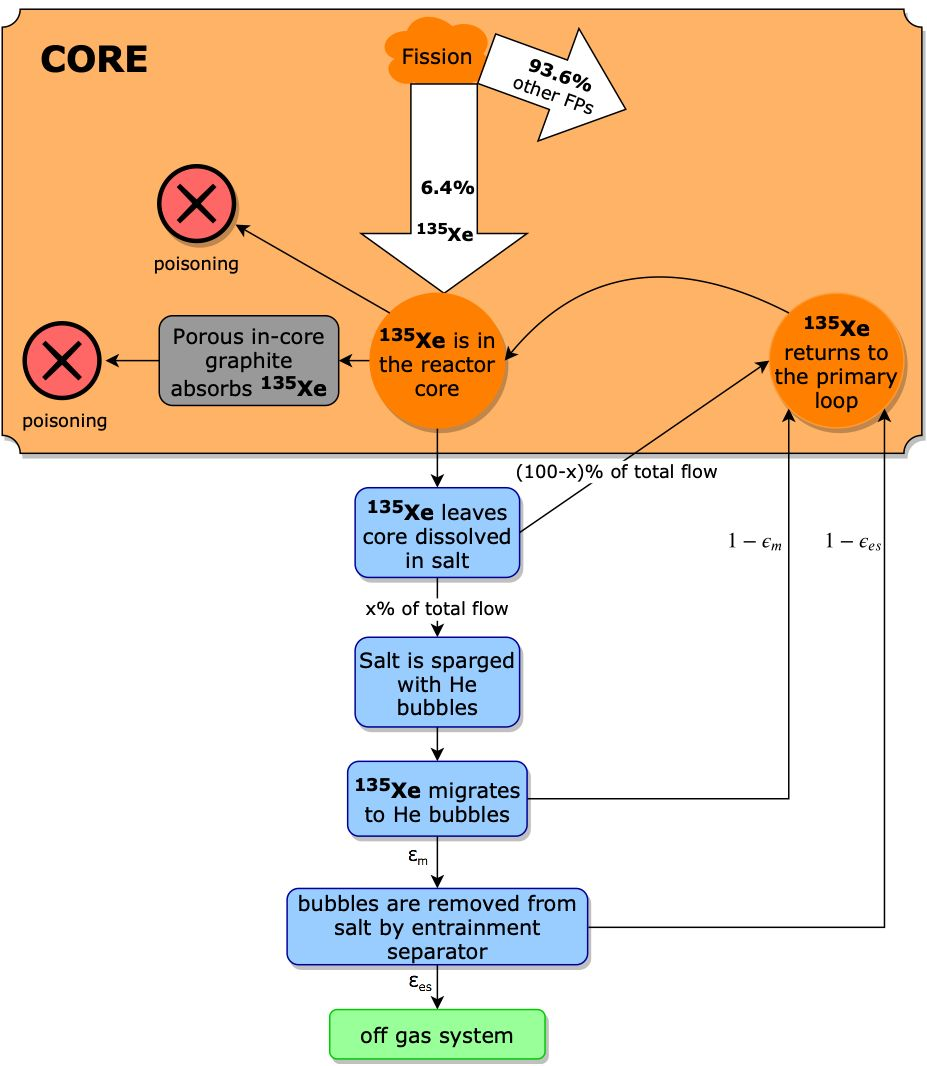
\includegraphics[width=0.6\textwidth]{principal_scheme.png}
        \end{center}
        \caption{Principal scheme of xenon removal from the salt.}
        \label{fig:scheme}
    \end{figure}

\subsubsection{Dakota}

    We used the Dakota code \cite{adams_dakota_2019} for sensitivity analysis 
    to assess the reactor performance at different load-follow scenarios when 
    the sparging system is enabled. The code provides optimization tools 
    including sensitivity analysis packages for miscellaneous design problems. 
    With Dakota group's words:

    \begin{quote}
        "In addition to its state-of-the-art optimization methods, Dakota
        includes methods for global sensitivity and variance analysis, 
            parameter
        estimation, uncertainty quantification, and verification, as well as
        meta-level strategies for surrogate-based optimization, hybrid
        optimization, and optimization under uncertainty."
    \end{quote}

    We performed a multidimensional parameter study by computing response data 
    sets for an n-dimensional hypergrid formed by sensitivity parameters. Each 
    sensitivity parameter is partitioned into equally-spaced intervals between 
    its upper and lower bounds. Each combination was then simulated by Saltproc 
    software coupled to Serpent.

\subsubsection{Serpent}

    Serpent software \cite{Lep2014} was used for Monte-Carlo based neutron 
    transport calculations. Serpent model with corresponding Serpent's 
    parameters stands on the MSBR design described in various reports prepared 
    for ARPA-E MEITNER Program \cite{rykhlevskii_fuel_2019, 
    rykhlevskii_modeling_2019, rykhlevskii_fuel_2020}.

\newpage
\FloatBarrier

\section{Sparging Design}

    A sparging system is composed of two separate components: Sparger (bubble 
    generator) and Separator (bubble separator). The role of the sparger is to 
    generate He bubbles in which noble gases diffuse while the role of the 
    separator is to remove bubbles from fuel salt which carry volatile noble 
    gases like Xe and Kr. The efficiency of the sparger component is expressed 
    in terms of gas removal efficiency ($\epsilon_{X}$) while that of the 
    separator is in terms of the bubble separation efficiency 
    ($\epsilon_{sep}$). Accordingly, total gas removal efficiency becomes 
    ${\epsilon^{X}}_{total} = \epsilon_{X} \times \epsilon_{sep}$ for any 
    target isotope $X$. A simple illustration of the system is given in Figure 
    \ref{fig:sparging}.

    \begin{figure}[htbp!]
        \begin{center}
            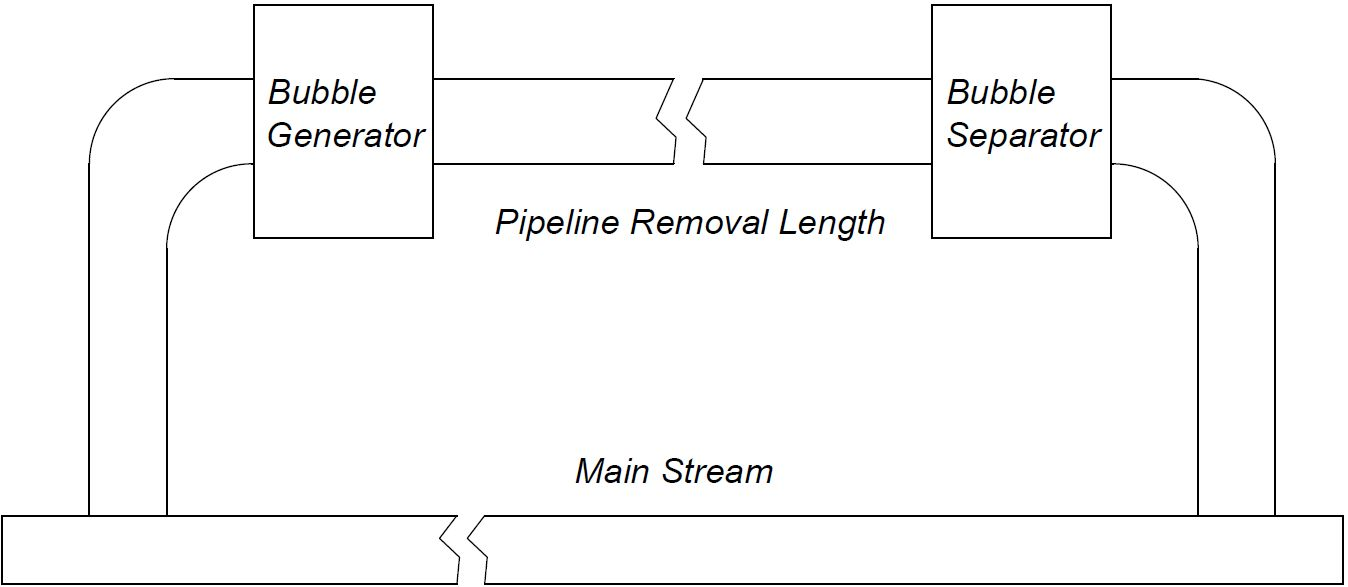
\includegraphics[width=0.8\textwidth]{bubble_separator_main.png}
        \end{center}
        \caption{Fission product removal system: Sparging}
        \label{fig:sparging}
    \end{figure}

\subsection{Sparger Design}

 As illustrated in Figure \ref{fig:sparging}, sparger includes a contactor 
 section and a long pipe with a contactor cross-section of $A_c = \pi\times 
 d^2/4$ and length of $L$. Gas removal efficiency in bubble generator is 
 defined by equation in Figure \ref{fig:eq2} based on 
 \cite{peebles_removal_1968}.

    \begin{figure}[h!]
        \begin{center}
            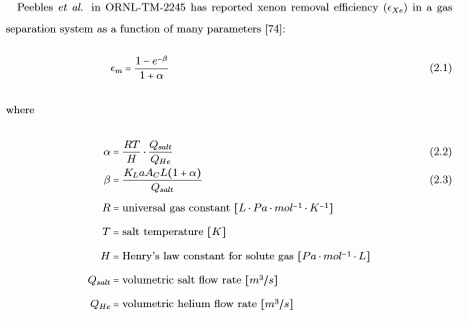
\includegraphics[trim={0 0 30 30}, clip, 
                width=1.0\textwidth]{eq2.1-part1.png}
            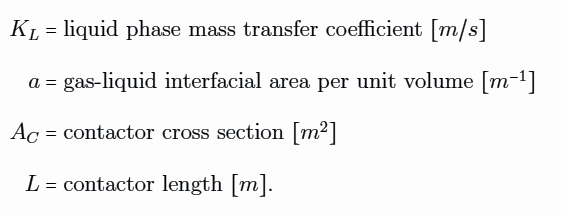
\includegraphics[width=0.7\textwidth]{eq2.1-part2.png}
        \end{center}
        \caption{Removal efficiency correlation from 
            \cite{peebles_removal_1968}}
        \label{fig:eq2}
    \end{figure}

    In the equation, gas-liquid interfacial area per unit volume ($a$) is:

    \begin{equation}\label{interfacial}
        a = \frac{6}{d_b} \frac{Q_{He}}{Q_{salt}+Q_{He}}
    \end{equation}

    Also, the universal gas constant is 8.314 L.Pa/mol-K, and Henry's law 
    constant is at the operating salt temperature. Gas constants for solute 
    gases of Xe, Kr, and H are then calculated at the operating salt 
    temperature based on a reference temperature of 298.15 K with the following 
    expression \cite{acp-15-4399-2015}:

    \begin{equation}\label{henry}
        H(T) = H(T_{ref})\times\exp(C(\frac{1}{T}-\frac{1}{T_{ref}}))
    \end{equation}
    where C denotes the exponential constant and the constants for Xe, Kr, and 
    H elements are 2300, 1900, and 0 K, respectively. Henry's law constants for 
    Xe, Kr, and H elements at the reference temperature are  4.3e-5, 2.5e-5, 
    and 2.6e-6 Pa/mol-L, respectively \cite{acp-15-4399-2015}.

    Liquid phase mass transfer coefficient ($K_L$) determined by the flow 
    dynamics is calculated by the following formula:

    \begin{equation}\label{kl}
        K_L = Sh \times D / d_p
    \end{equation}
    where $D$ is the liquid phase diffusivity of 2.5e-9 (cm$^2$/s) (from CFD 
    group), $Sh$ is the Sherwood number, and $d_p$ is the pipe diameter. The 
    dimensionless $Sh$ number developed in Milestone 1.2 is defined as follows:

    \begin{equation}\label{sh}
        Sh = 2.06972 * Re_D^{0.555} * Sc^{0.5}
    \end{equation}
    where $Re_D$ is the pipe Reynolds number and $Sc$ is the dimensionless 
    Schmidt number defined in \ref{sc}:

    \begin{equation}\label{sc}
        Sc = \nu/D
    \end{equation}
    where $\nu$ is the kinematic viscosity ($\mu/\rho$) in m$^2$/s. Here, for 
    the calculation of the pipe Reynolds number, we used

    \begin{equation}\label{reynold}
        Re_D = \frac{Dv}{\nu}
    \end{equation}
    where $v$ denotes the fluid velocity in m/s. Temperature-dependent density 
    and dynamic viscosity of the fluid were supplied by the CFD group and are 
    defined in Eq. \ref{density} and \ref{viscosity}:

    \begin{equation}\label{density}
        \rho = 6.105 - 0.001272 * T [kg/m^3]
    \end{equation}
    and
    \begin{equation}\label{viscosity}
        \mu = 1.076111581E-2 * (T / 1000)**(-4.833549134) [N.s/m^2]
    \end{equation}
    where T is the salt temperature in Kelvin.

    In a sparger model, the parameters need to be designed are $Q_{salt}$, 
    $Q_{He}$, $L$, $d_p$, $d_b$, and $T_{salt}$.

\newpage
\FloatBarrier

\subsection{Separator Design}

    A detailed design of the separator is given in Figure 
    \ref{fig:bubble_sprt}. We employed the regression model for the estimation 
    of the bubble separation efficiency developed within the scope of Milestone 
    1.2.

    The model given in Figure \ref{fig:reg_model} is expressed in terms of gas 
    outlet diameter ($D_o$), sparger (pipe) diameter ($D$), bubble diameter 
    ($d_b$), pressure difference ($\Delta p$) between the inlet and the gas 
    outlet, liquid superficial velocity ($j_l$), salt density ($\rho$), nominal 
    void fraction ($\alpha$ = $j_g/(j_{l}+j_{g})$ or 
    $Q_{He}/(Q_{salt}+Q_{He})$), slope of the initial swirling ($k$), cone 
    diameter of the recovery vane ($D_c$ = 3.41 $D_o$), and the pipe Reynolds 
    number ($Re_D$) calculated by Eq. \ref{reynold}. Liquid superfical velocity 
    ($j_l$) is calculated from volumetric salt flow rate in the following way: 
    $j_l = Q_{salt}/A$ where $A = \pi\times D^2/4$ is the contactor 
    cross-sectional area.

    In a separator model, the parameters need to be designed are $Q_{salt}$, 
    $Q_{He}$, $D_o$, $d_p$, $d_b$, $\Delta p$, and $T_{salt}$.

    \begin{figure}[htbp!]
        \begin{center}
            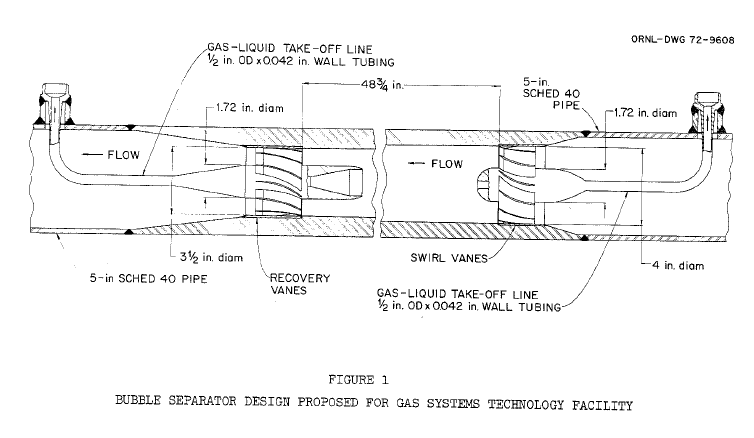
\includegraphics[width=\textwidth]{bubble_separator_detailed.png}
        \end{center}
        \caption{Entrainment Separator}
        \label{fig:bubble_sprt}
    \end{figure}

    \begin{figure}[htbp!]
        \begin{center}
            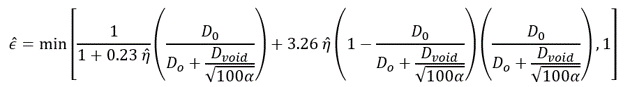
\includegraphics[width=1.1\textwidth]{sep_eff_eq_1.png}
            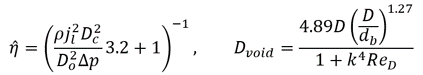
\includegraphics[width=0.7\textwidth]{sep_eff_eq_2.png}
        \end{center}
        \caption{Regression model from Milestone 1.2 report}
        \label{fig:reg_model}
    \end{figure}

\newpage
\FloatBarrier

\subsection{Integration to Saltproc}

    Sparging system was embedded to Saltproc by separately defining Sparger and 
    Separator clasesses. \textit{read\_processes\_from\_input} function in 
    \textit{app.py} script calls the classes to calculate removal efficiencies 
    of target elements. More information about Saltproc functions and classes 
    can be found in Milestone 2.1 report \cite{rykhlevskii_milestone_2019} and 
    ARFC Github repo (https://github.com/arfc/saltproc). Sparger class uses the 
    equation in Figure \ref{fig:eq2} whereas Separator uses the equation in 
    Figure \ref{fig:reg_model}. In this way, besides the existing flexibility, 
    saltproc now enables Sparging system when the "self" input key is used in 
    the json object input file.

    Later, these equations are to be replaced with improved ones as the 
    experimental and simulation data are supplied by the project's research 
    groups.

\newpage
\FloatBarrier

\section{Sensitivity Analysis}

    To design a feasible sparging system, we performed two separate sensitivity 
    analyses:

    \begin{enumerate}
        \item Reactor core behavior at different load-follow transients and 
                decision on how much removal efficiency is needed to maintain 
                    the criticality in the MSBR when the sparging system is 
                    enabled.
        \item Specification and optimization of design boundaries for the 
                sparger and separator.
    \end{enumerate}

    Results of these analyses were later combined to understand the ultimate 
    design boundaries of sparging system.

\subsection{Load-Follow Transients}

    Figure \ref{fig:workflow} illustrates a simplified workflow of the 
    sensitivity analysis for the assessment of the reactor core behavior. 
    Results define total $\varepsilon$$_{Xe}$ requirements for prototype Xe 
    sparger and entrainment separator system.

    \begin{figure}[htbp!]
        \begin{center}
            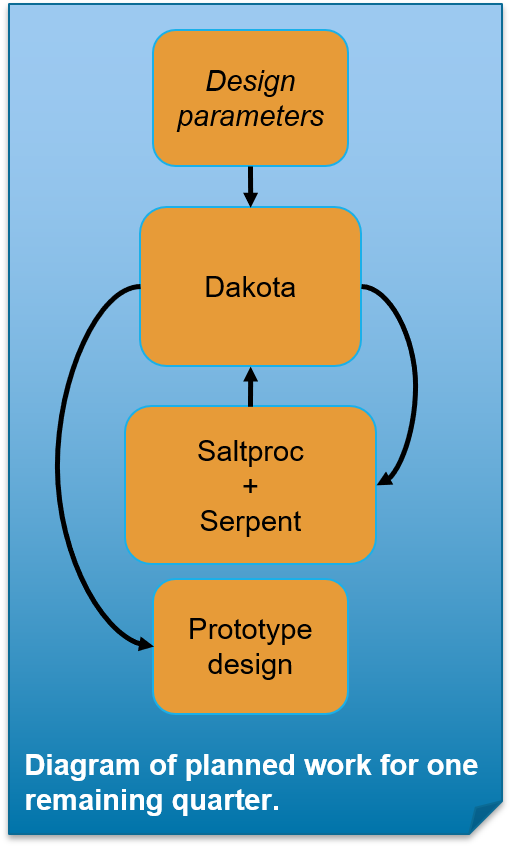
\includegraphics[width=0.35\textwidth]{workflow.png}
        \end{center}
        \caption{Sensitivity analysis workflow.}
        \label{fig:workflow}
    \end{figure}

\subsubsection{Scenarios}

    Two critical load following scenarios were investigated:
    \begin{itemize}
        \item The first worst-case scenario simulates 8 hours at full power 
                after an 8-hour shutdown, providing maximum Xe poisoning effect 
                    in the reactor.
        \item The second worst-case scenario considers a short period 
                load-follow for maximum Xe accumulation over time. In this 
                    scenario, the reactor runs at full power for one hour after 
                    an hour of shutdown, and this repeats several times.
    \end{itemize}

\subsubsection{Sensitivity Parameters}

    We considered the Xe removal efficiency ($\varepsilon$$_{Xe}$) given in 
    Figure \ref{fig:eq2} and the bubble separation efficiency given in Figure 
    \ref{fig:reg_model}, ranging from 0 to 100 \%, as input variables to the 
    Saltproc code. We used k$_{eff}$, $\beta$$_{eff}$, breeding ($\gamma$) and 
    reactivity feedbacks ($\alpha$) as performance metrics. As the development 
    of an experimental correlation to define the bubble separation efficiency 
    of the separator was continued by the CFD group at the moment when we 
    performed this study, we assumed it as 95\%. Note that this value is 
    expected to be between 95 and 100\%.

    Other parameters used in Figure \ref{fig:eq2} to calculate the removal 
    efficiency are as follow: length ($L$) = 11 m, diameter ($d_p$) = 0.4 m, 
    volume ($V$) = 1.4 m$^{3}$, A$_c$ = 0.126 m$^{2}$, He bubble diameter, 
    d$_b$ = 0.508 mm, salt volumetric flow rate ($Q_{salt}$) = 2 m$^{3}$/s, 
    sparging gas (helium) volumetric flow rate ($Q_{He}$) = 0.1 m$^{3}$/s.

\subsection{Sparging System}

    As a final step of the sensitivity analysis for the sparging system, we 
    bounded sparging system design based on the load-following results. For 
    bubble generator (sparger), we explored the effect of sensitivity (design) 
    parameters on gas removal efficiencies of Xe, Kr, and H target elements. In 
    the case of spearator, we considered the bubble separator efficiency.

    To understand the interdependencies of design parameters, we examined 
    individual and binary effects of sparger design parameters on the Xe 
    removal efficiency.

\subsubsection{Sensitivity Parameters}

    Design parameters for sparging system were considered as salt volumetric 
    flow rate ($Q_{salt}$), helium volumetric flow rate ($Q_{He}$), bubble 
    diameter ($d_b$), pipe diameter ($d_p$), pipe length ($L$), pressure 
    difference ($\Delta p$), gas outlet diameter ($D_o$), and salt temperature 
    ($T_{salt}$). The metrics corresponding to the performance of the system 
    are gas removal efficiencies ($\varepsilon$$_{X}$) of the sparger where 
    $_{X}$ denotes Xe, Kr, and H target elements and the bubble separation 
    efficiency of the separator ($\varepsilon$$_{sep}$).

    Base design parameters (supplied by the CFD group) used for comparison in 
    the sensitivity analysis are as follow: pipe length ($L$) = 10 m, pipe 
    diameter ($d_p$) = 0.1 m, bubble diameter ($d_b$) = 1 mm, salt volumetric 
    flow rate ($Q_{salt}$) = 0.1 m$^{3}$/s, salt temperature ($T_{salt}$) = 900 
    K, pressure difference ($\Delta p$) = 4e5 Pa, gas outlet diameter ($D_o$) = 
    0.02, and helium volumetric flow rate ($Q_{He}$ = 5\% of $Q_{salt}$) = 
    0.005 m$^{3}$/s. Accordingly, we changed these parameters between -50\% and 
    +50\% (i.e., $\pm$10\%, $\pm$25\% and $\pm$50\%).

\newpage
\FloatBarrier

\section{Results}

\subsection{Load-Follow}

    We first carried out sensitivity analysis for different load-follow 
    transients. Initial results shown in Figure \ref{fig:loadfollow} and the 
    results from the previous work \cite{rykhlevskii_fuel_2020} point out that 
    MSBR cannot do load-follow without gas removal at BOL (30 days), MOL (15 
    years), and EOL (30 years) as the effective multiplication factor decreases 
    with the start of the shutdown. Online gas removal from the fuel salt even 
    with moderate efficiency significantly reduces the xenon poisoning effect, 
    yet very high removal efficiency seems unnecessary to negate the negative 
    effect of xenon poisoning. Load-follow at EOL is the worst for k$_{eff}$ 
    and consequently considered for sensitivity analysis.

    \begin{figure}[h]
        \begin{center}
            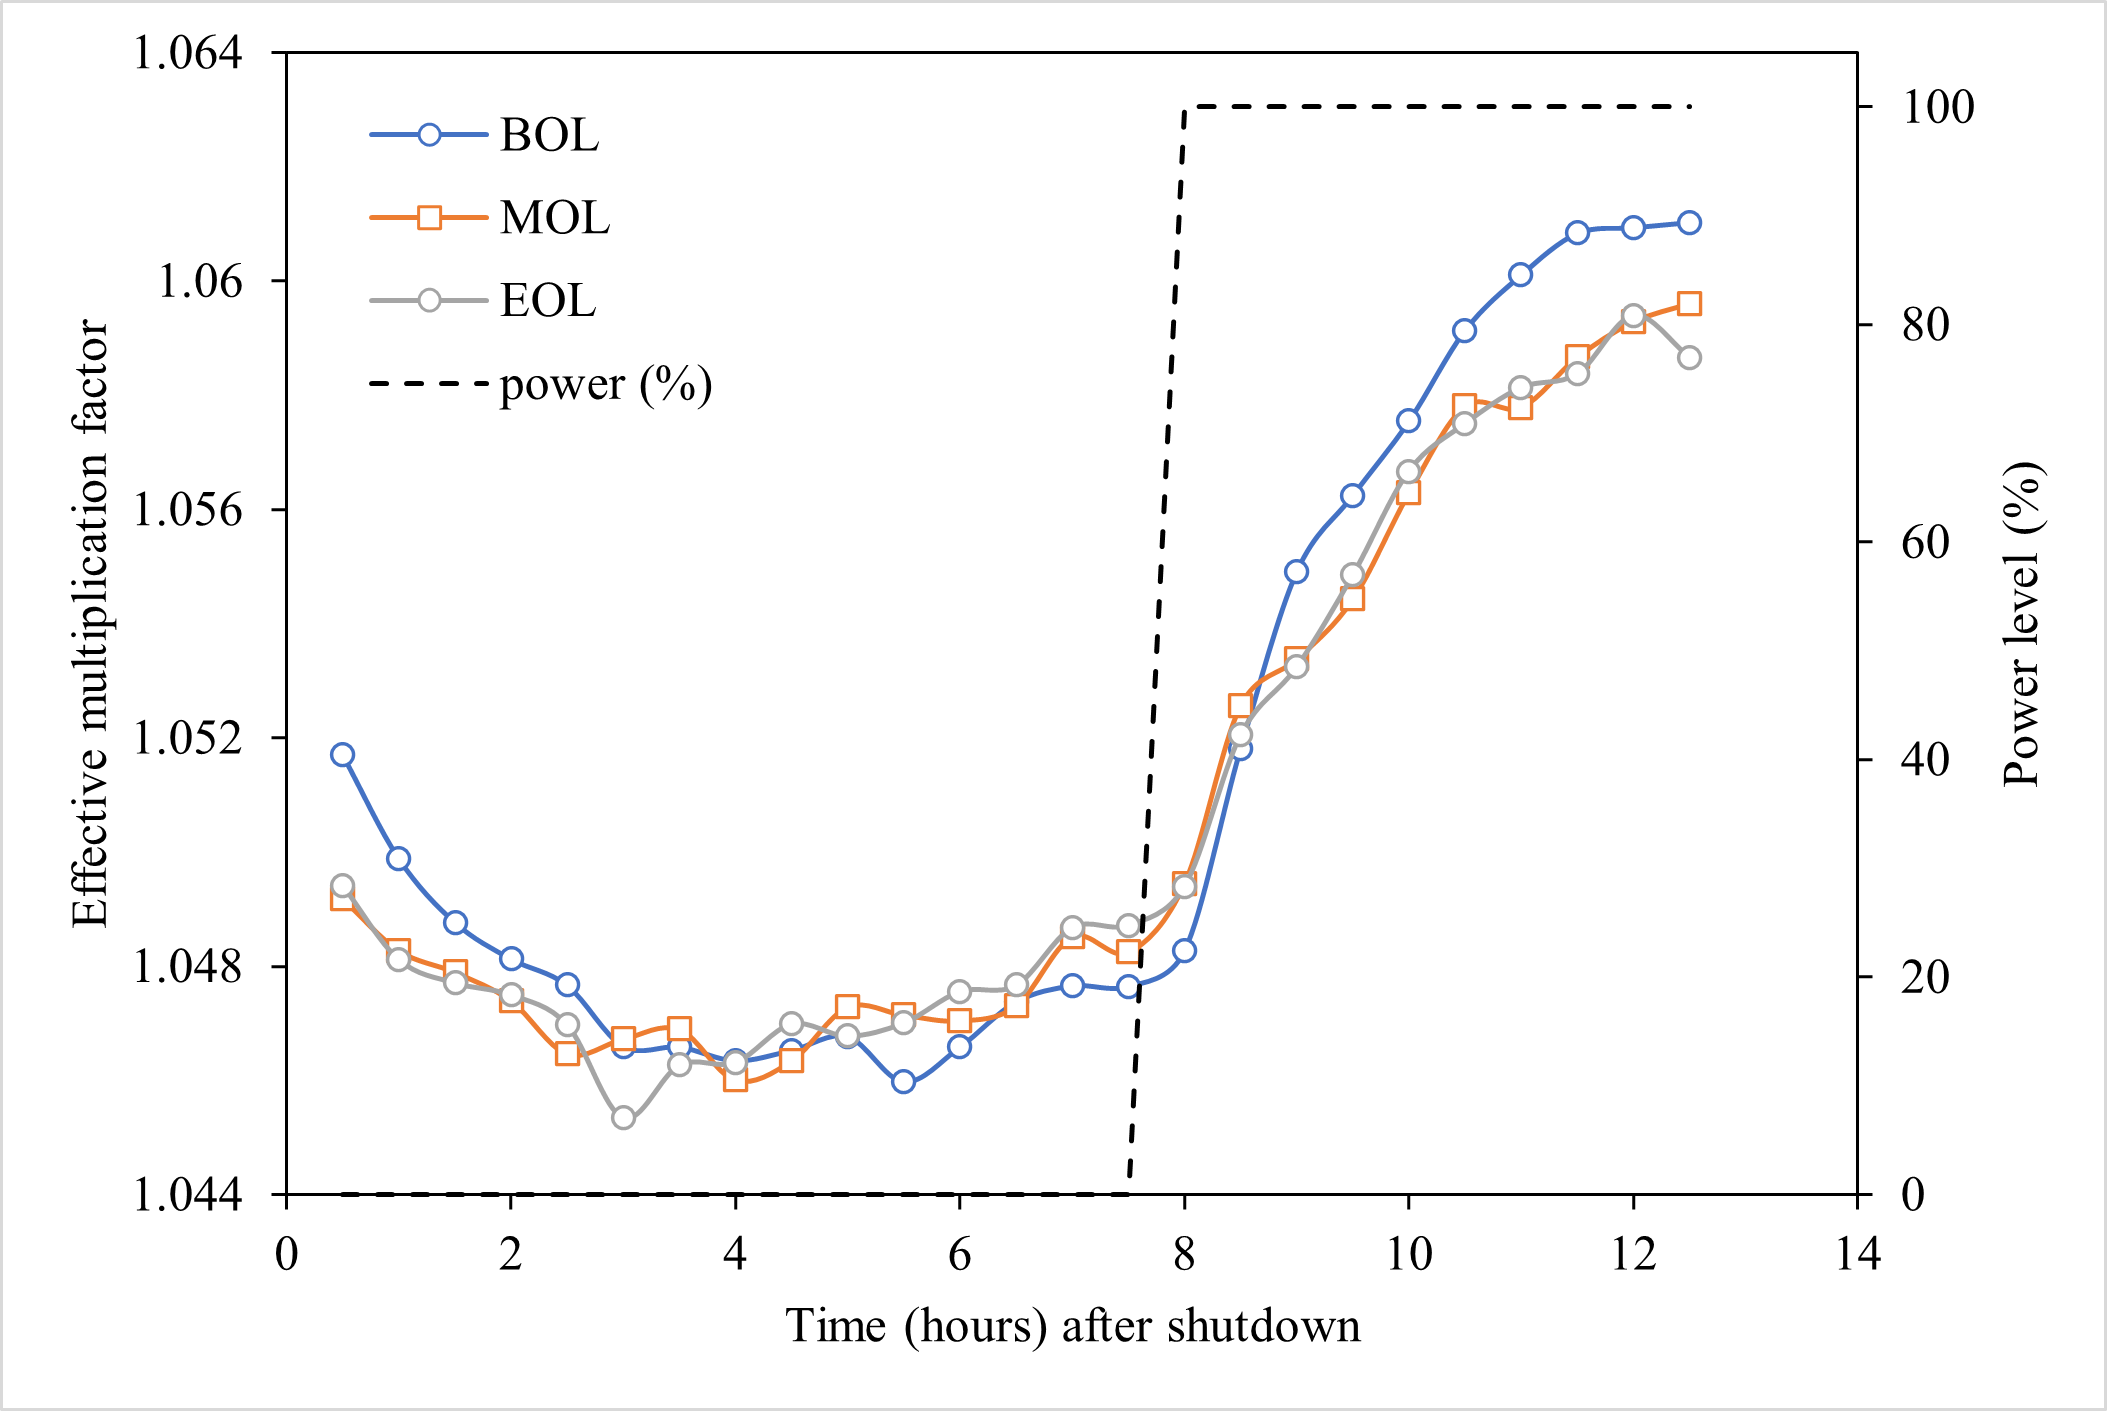
\includegraphics[width=1.0\textwidth]{msbr_loadfollow.png}
        \end{center}
        \caption{Load follow is attempted at BOL (30 days), MOL (15 years) and 
            EOL (30 years) without gas removal system. Uncertainty in k$_{eff}$ 
            is 25 pcm. 30 mins time resolution.}
        \label{fig:loadfollow}
    \end{figure}

\subsubsection{First Scenario}

    Figure \ref{fig:single_keff} shows the results of the first scenario 
    (single load-follow) for k$_{eff}$. After a lifetime of operation at 
    $\varepsilon$$_{Xe}$ = 0.536, single load-follow was attempted. In this 
    transient, for the base case geometry, the reactor can recover from the Xe 
    poisoning effect after $\varepsilon$$_{Xe}$ = 26.8\%. Generally, increasing 
    gas removal efficiency increases excess reactivity. If higher efficiency is 
    used, then the reactor recovers excess reactivity quicker, within a few 
    hours.

    As to the breeding ratio depicted in Figure \ref{fig:single_breed}, single 
    load-follow transient results in a gradual decrease. Increasing the gas 
    removal efficiency slightly lowers the breeding ratio during the 
    load-follow.

    For the delayed neutron fraction ($\beta$$_{eff}$) given in Figure 
    \ref{fig:single_delayed}, we observed no significant change. Instead, 
    $\beta$$_{eff}$ fluctuates in a narrow range due to the statistical 
    deviation.

    We also explored multiple consecutive load-follow transients causing sharp 
    changes in salt composition. As can be clearly seen in Figure 
    \ref{fig:double_keff}, k$_{eff}$ begins fluctuating with Xe buildup and 
    burndown period. We understand from the result that to keep the reactor 
    stable, gas removal efficiency at least $\varepsilon$$_{Xe}$ = 53.6\% is 
    required (corresponds in base case geometry to K$_{L}$ $>$ 25 ft/hr = 2.117 
    mm/s).

    With the same load-follow period, we increased the number of transients. We 
    saw from Figure \ref{fig:triple_keff} that a higher gas removal efficiency 
    (at least $\varepsilon$$_{Xe}$ = 76.9\% or K$_{L}$ $>$ 50 ft/hr = 4.233 
    mm/s) is needed to keep the reactor stable. Therefore, these results 
    indicated that as the number of power ramps increases, a higher gas removal 
    efficiency is required for stable reactor behavior.

    \begin{figure}[htbp!]
        \begin{center}
            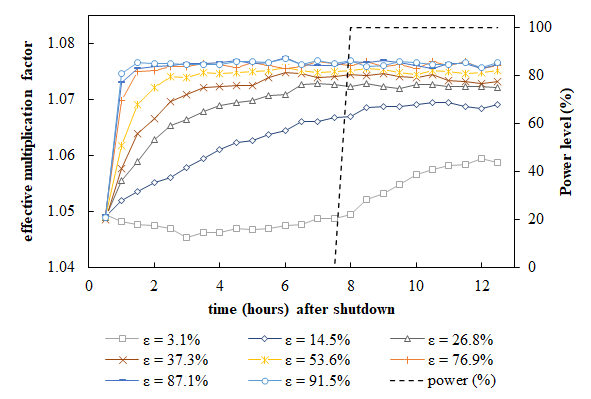
\includegraphics[width=0.8\textwidth]{single_ramp_keff.png}
        \end{center}
        \caption{After a lifetime of operation at $\varepsilon$$_{Xe}$= 0.536, 
            load follow is attempted at EOL. Above shows k$_{eff}$ during load 
            follow transient for various total Xe removal efficiencies
        ($\varepsilon$$_{Xe}$) over time after shutdown.}
        \label{fig:single_keff}
    \end{figure}

    \begin{figure}[htbp!]
        \begin{center}
            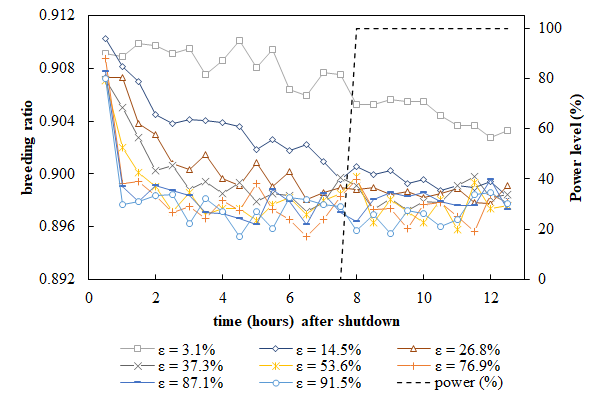
\includegraphics[width=0.8\textwidth]{single_ramp_breeding.png}
        \end{center}
        \caption{After a lifetime of operation at $\varepsilon$$_{Xe}$= 0.536, 
            load follow is attempted at EOL. Above shows breeding ratio during 
            load
        follow transient for various total Xe removal efficiencies
        ($\varepsilon$$_{Xe}$) over time after shutdown.}
        \label{fig:single_breed}
    \end{figure}

    \begin{figure}[htbp!]
        \begin{center}
            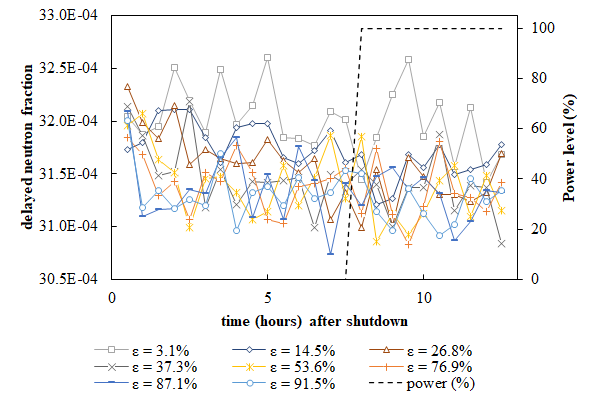
\includegraphics[width=0.8\textwidth]{single_ramp_delayed.png}
        \end{center}
        \caption{After a lifetime of operation at $\varepsilon$$_{Xe}$= 0.536, 
            load follow is attempted at EOL. Above shows $\beta$$_{eff}$ during 
            load
        follow transient for various total Xe removal efficiencies
        ($\varepsilon$$_{Xe}$) over time after shutdown.}
        \label{fig:single_delayed}
    \end{figure}

    \begin{figure}[htbp!]
        \begin{center}
            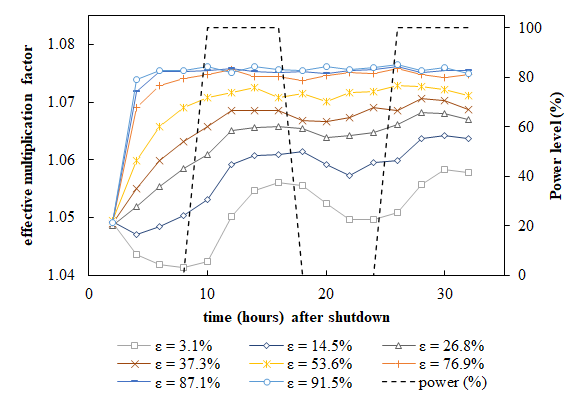
\includegraphics[width=0.8\textwidth]{double_ramp_keff.png}
        \end{center}
        \caption{After a lifetime of operation at $\varepsilon$$_{Xe}$= 0.536, 
            load follow is attempted at EOL. Above shows k$_{eff}$ during 
            multiple load follow transient for various total Xe removal 
            efficiencies
        ($\varepsilon$$_{Xe}$) over time after shutdown.}
        \label{fig:double_keff}
    \end{figure}

    \begin{figure}[htbp!]
        \begin{center}
            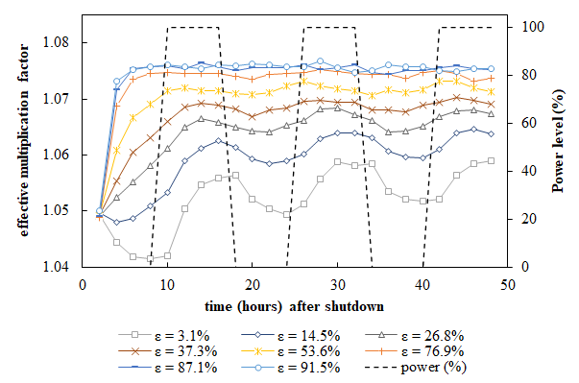
\includegraphics[width=0.8\textwidth]{triple_ramp_keff.png}
        \end{center}
        \caption{After a lifetime of operation at $\varepsilon$$_{Xe}$= 0.536, 
            load follow is attempted at EOL. Above shows  k$_{eff}$ during 
            multiple load follow transient for various total Xe removal 
            efficiencies
        ($\varepsilon$$_{Xe}$) over time after shutdown.}
        \label{fig:triple_keff}
    \end{figure}

\newpage
\FloatBarrier

\subsubsection{Second Scenario}

    Unlike the previous load-follow transients, in this part, we examined short 
    period load-follow transients (second scenario) and implemented four 
    consecutive power ramps. As can be seen in Figure \ref{fig:quadro_keff}, we 
    saw a quick recovery from shutdown even with low gas removal efficiency.

    \begin{figure}[htbp!]
        \begin{center}
            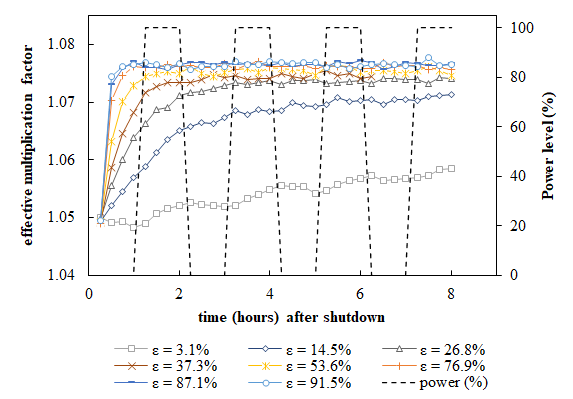
\includegraphics[width=0.9\textwidth]{quadro_ramp_keff.png}
        \end{center}
        \caption{After a lifetime of operation at $\varepsilon$$_{Xe}$= 0.536, 
            load follow is attempted at EOL. Above shows  k$_{eff}$ during 
            multiple load follow transient for various total Xe removal 
            efficiencies
        ($\varepsilon$$_{Xe}$) over time after shutdown.}
        \label{fig:quadro_keff}
    \end{figure}

\newpage
\FloatBarrier

\subsection{Sparging System}

    The results of the previous section directly pointed to a sparging system 
    design adaptable to different load-follow scenarios. This system design 
    should cover a wide range of efficiency as high as 80\% (corresponds to the 
    triple load-follow). We will, therefore, separately handle the sparger and 
    separator designs in this context.

\subsubsection{Sparger Design}

    First of all, we sought potential sparger designs around the base design 
    and changed the considered parameters of the base design up to $\pm$ 50\%. 
    Figure \ref{fig:individual_eff_sparger} and \ref{fig:binary_eff_sparger} 
    show change in Xe removal efficiency. From the binary effects, we can say 
    that each design parameter is acting independently on the removal 
    efficiency. This is because the sub-plots indicate a non-convex structure 
    and any parameter (in x and y axes) on any subplot either always increases 
    or decreases the removal efficiency.

    When we look at the individual effects on sparger design, gas removal 
    efficiencies decrease with increasing bubble diameter and salt flow rate 
    whereas gas removal efficiencies increase with increasing pipe diameter, 
    pipe length, helium flow rate, and salt temperature.

    In addition, due to the different thermo-dynamics and chemical properties 
    of the target elements, the change of tritium removal efficiency somewhat 
    different from that of Xe and Kr removal efficiency, being affected 
    significantly by salt temperature change.

    Furthermore, salt temperature and sparger pipe diameter look like not 
    effective players in the adjustment of the gas removal efficiency as the 
    10\% increase in temperature only results in about 3\% increase in 
    efficiency. Even with 50\% change, there is only a 10\% gain in efficiency, 
    by increasing from 40\% to about 45\%. In addition, we may need an 
    additional heater before sparger to elevate the salt temperature as the 
    salt temperature is determined by the reactor design itself.

    \begin{figure}[htbp!]
        \begin{center}
            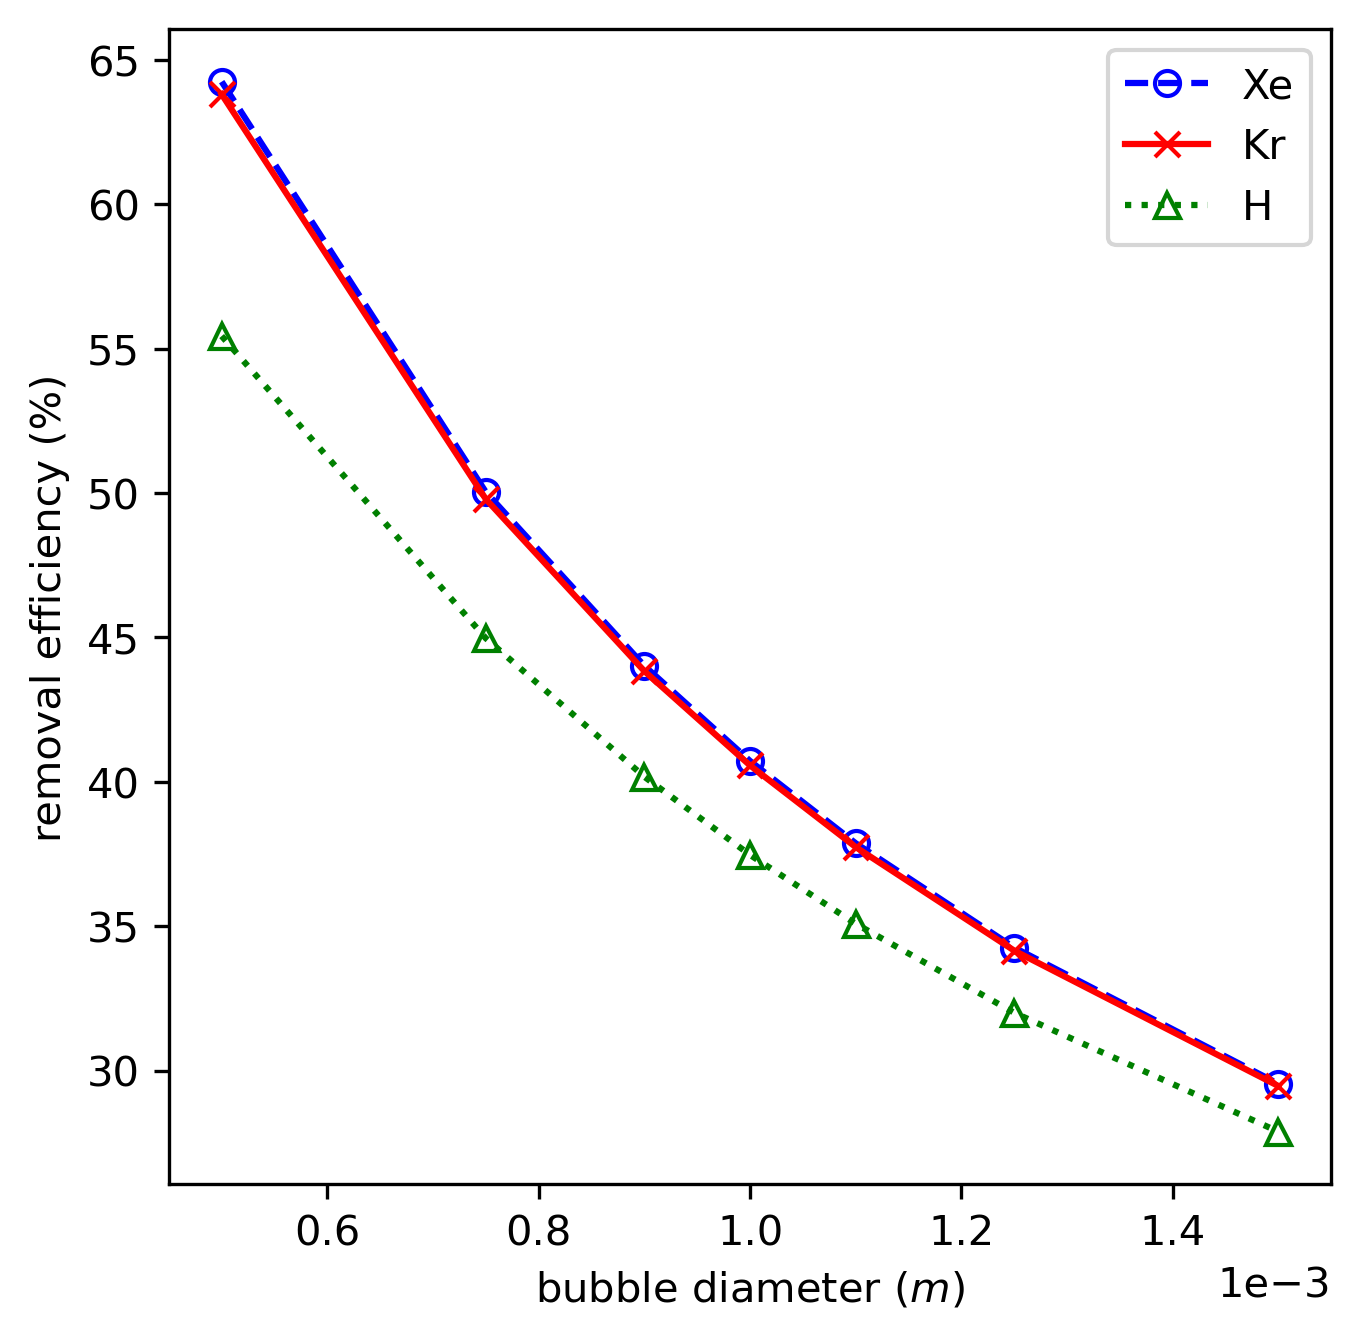
\includegraphics[width=0.45\textwidth]{Sparger_Xe_eff_vs_db.png}
            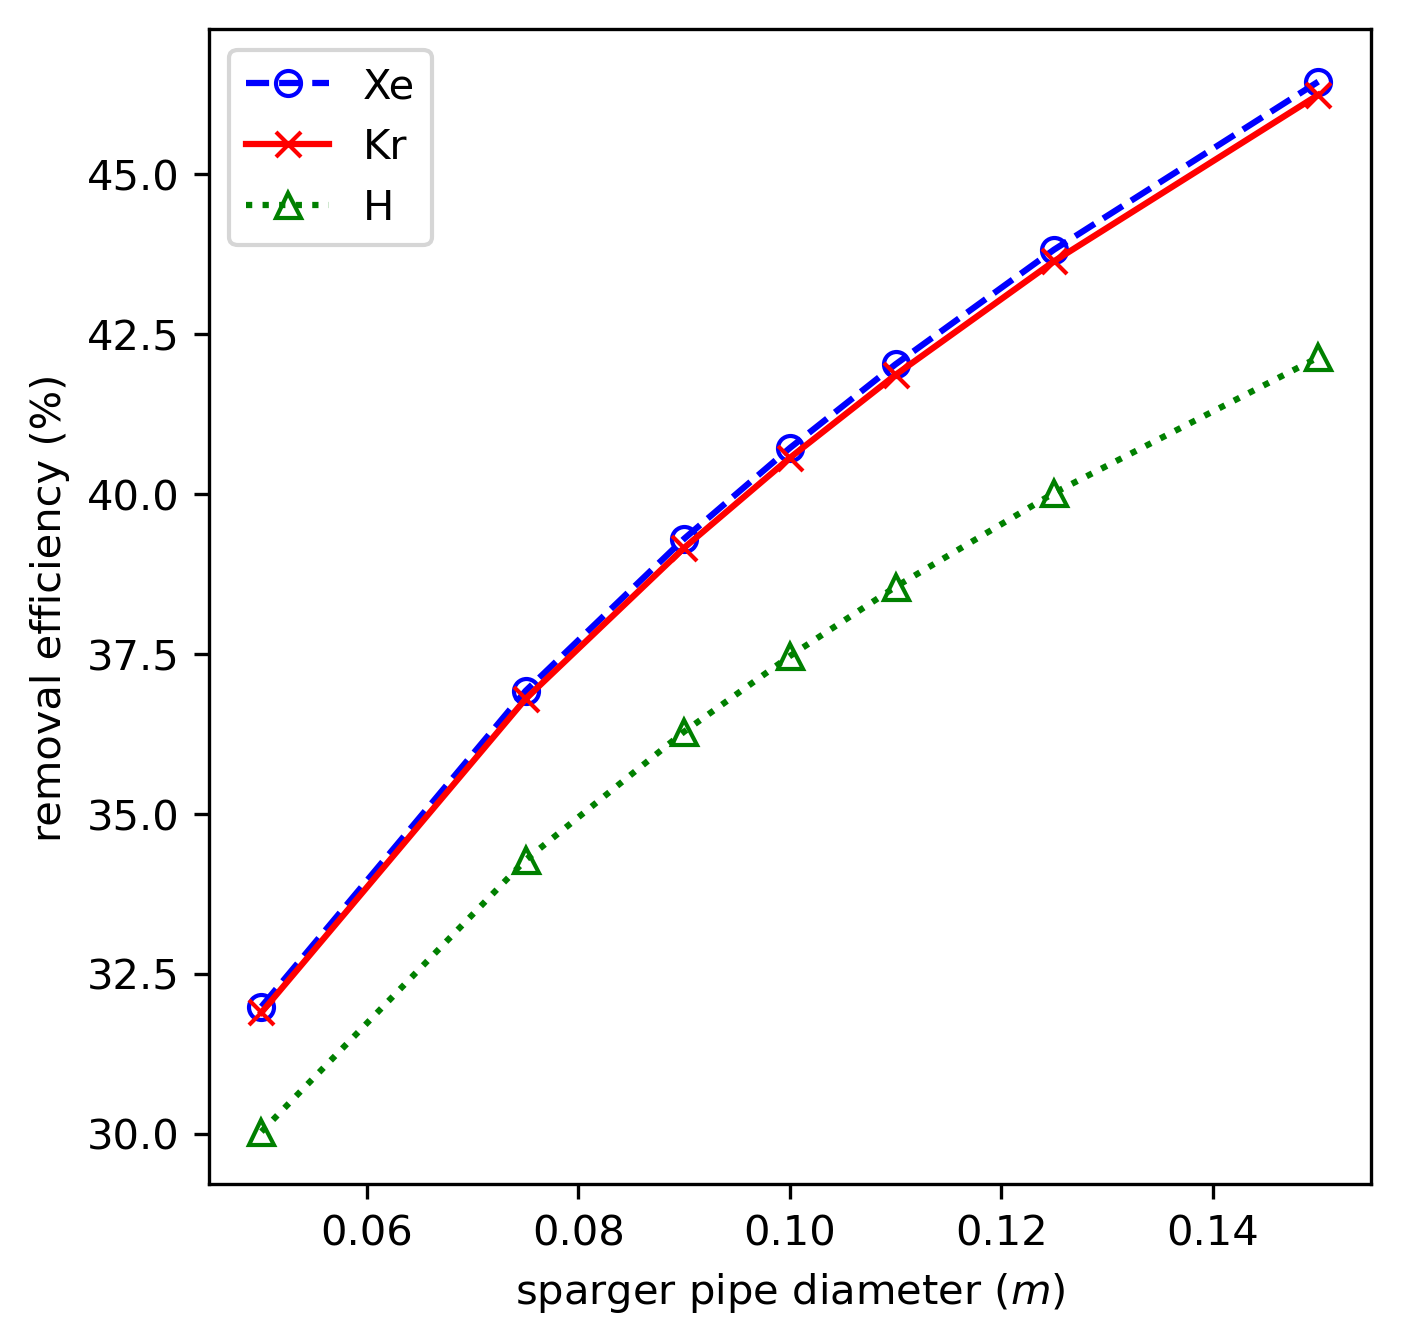
\includegraphics[width=0.45\textwidth]{Sparger_Xe_eff_vs_dp.png}
            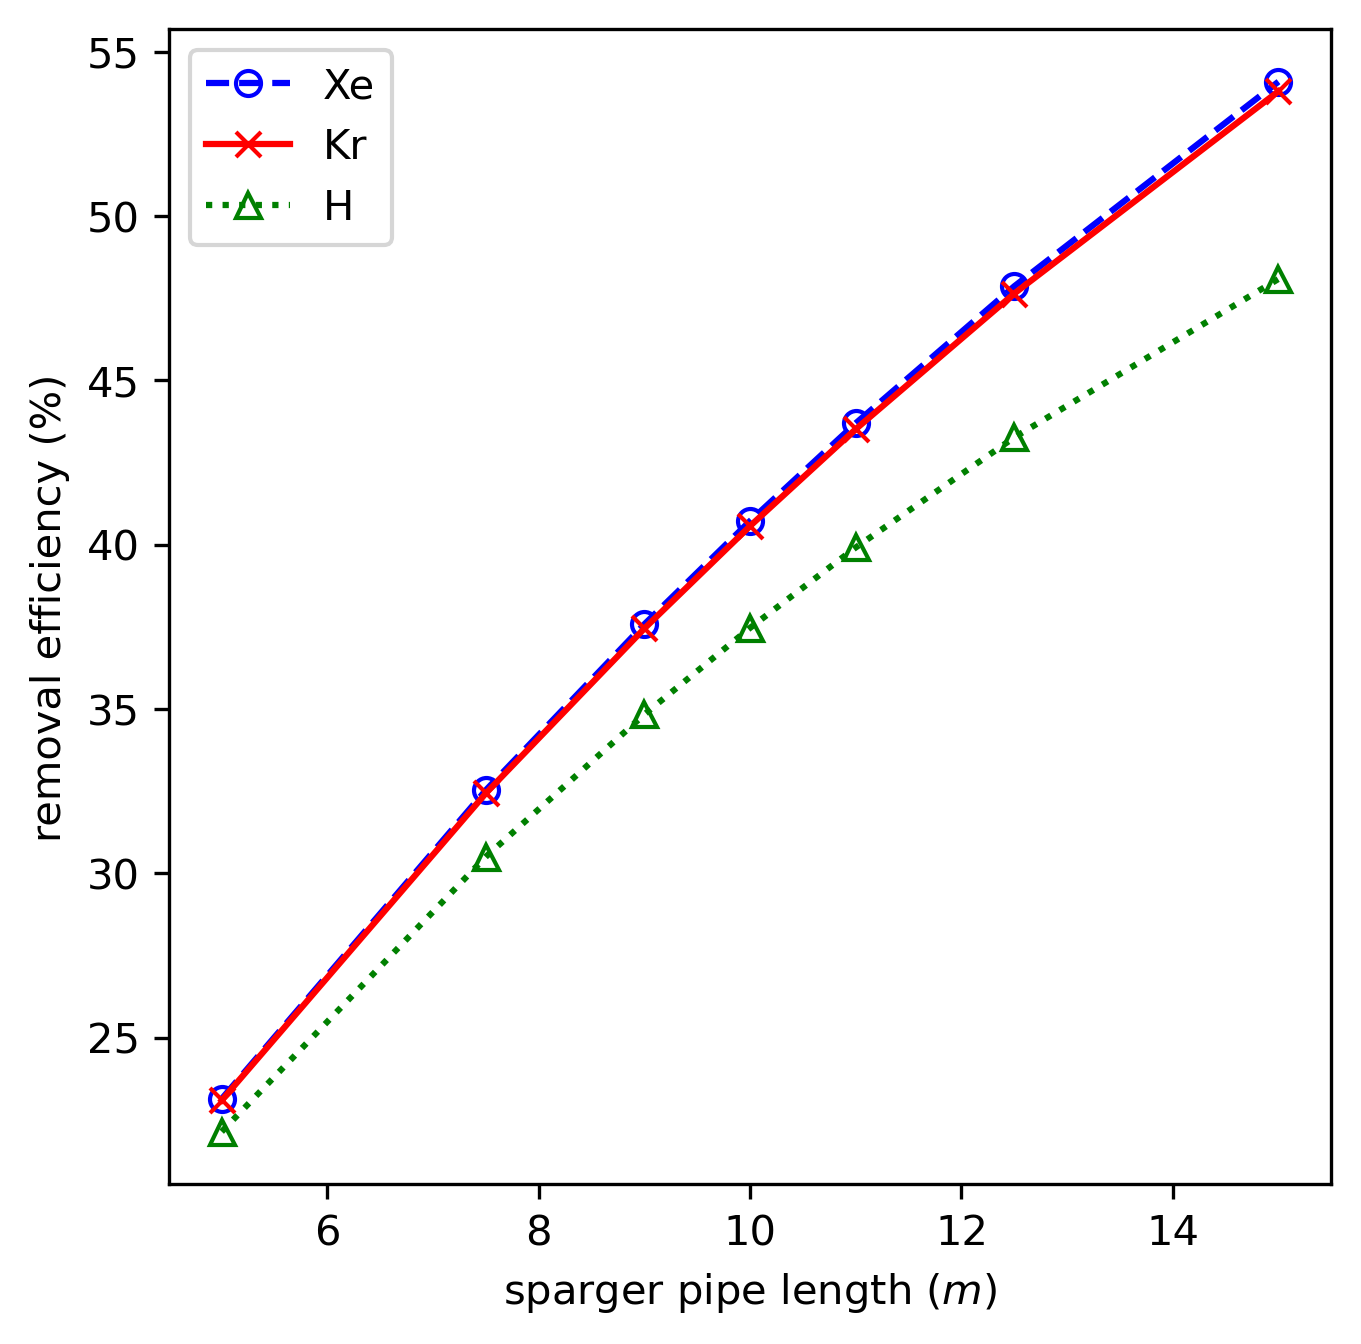
\includegraphics[width=0.45\textwidth]{Sparger_Xe_eff_vs_length.png}
            \includegraphics[width=0.45\textwidth]{Sparger_Xe_eff_vs_Q_salt.png}
            \includegraphics[width=0.45\textwidth]{Sparger_Xe_eff_vs_Q_He.png}
            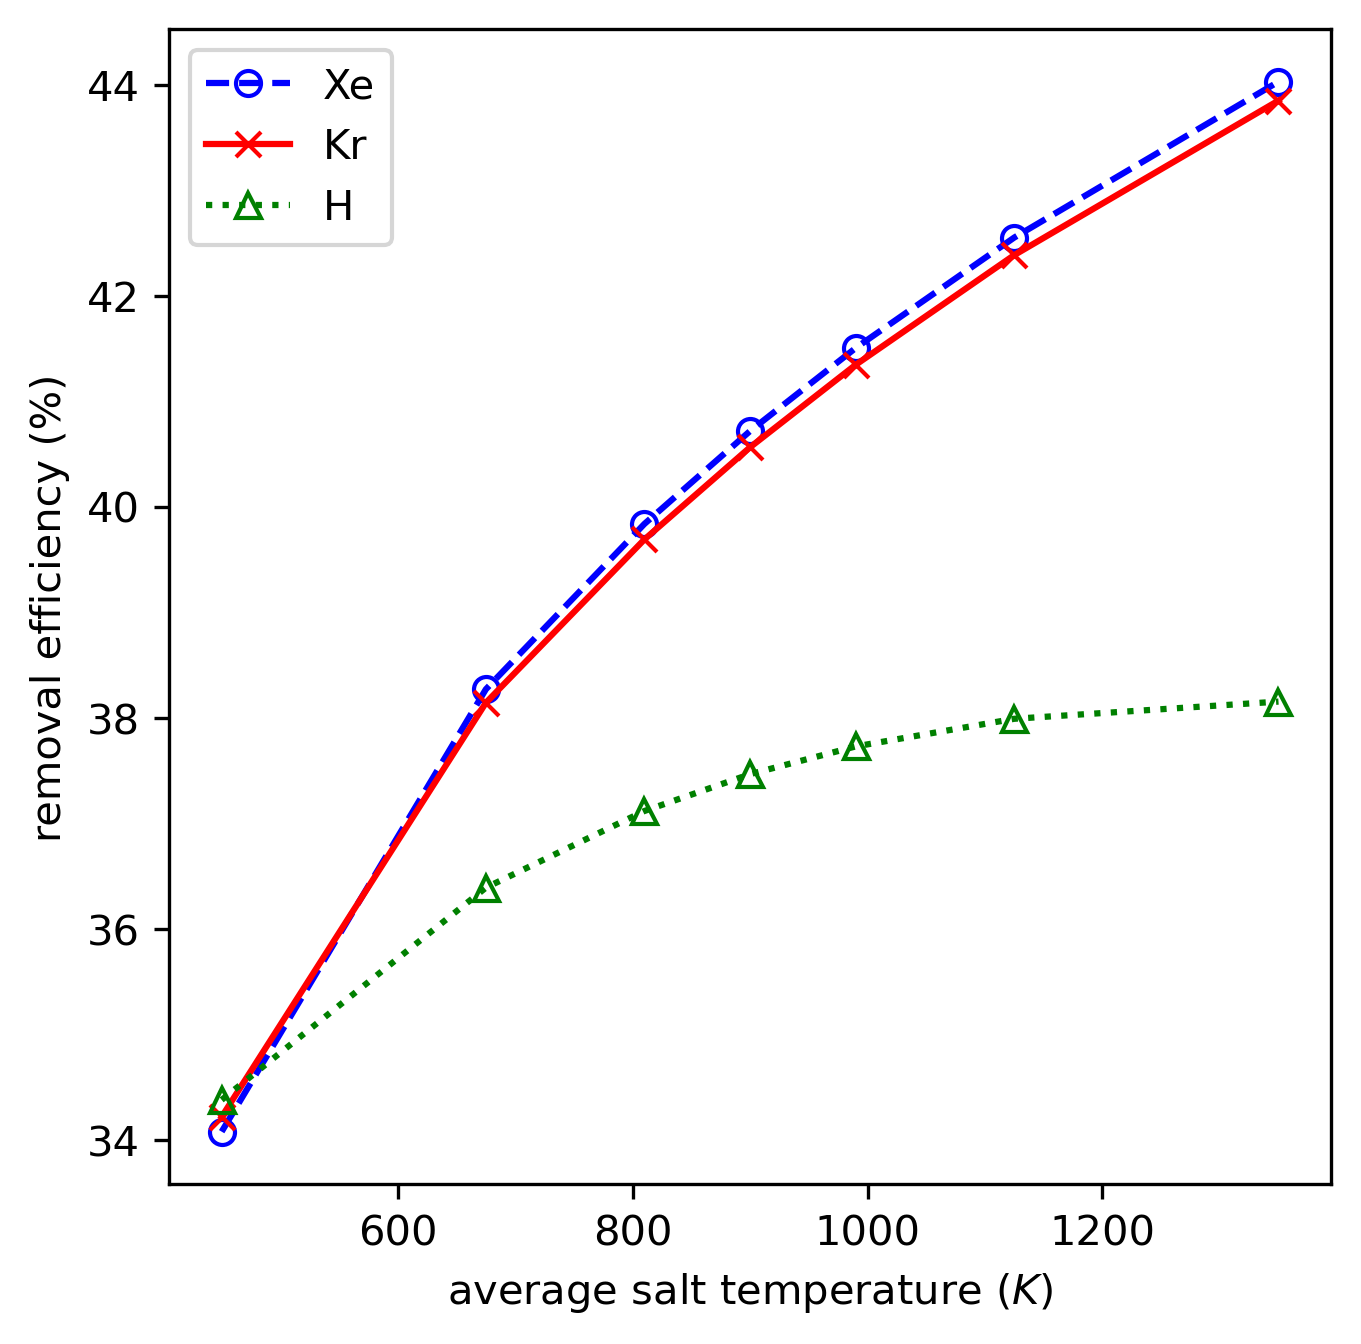
\includegraphics[width=0.45\textwidth]{Sparger_Xe_eff_vs_temp_salt.png}
        \end{center}
        \caption{Individual effect of design parameters on the Xe removal 
            efficiency ($\varepsilon$$_{Xe}$).}
        \label{fig:individual_eff_sparger}
    \end{figure}

    \begin{figure}[htbp!]
        \begin{center}
            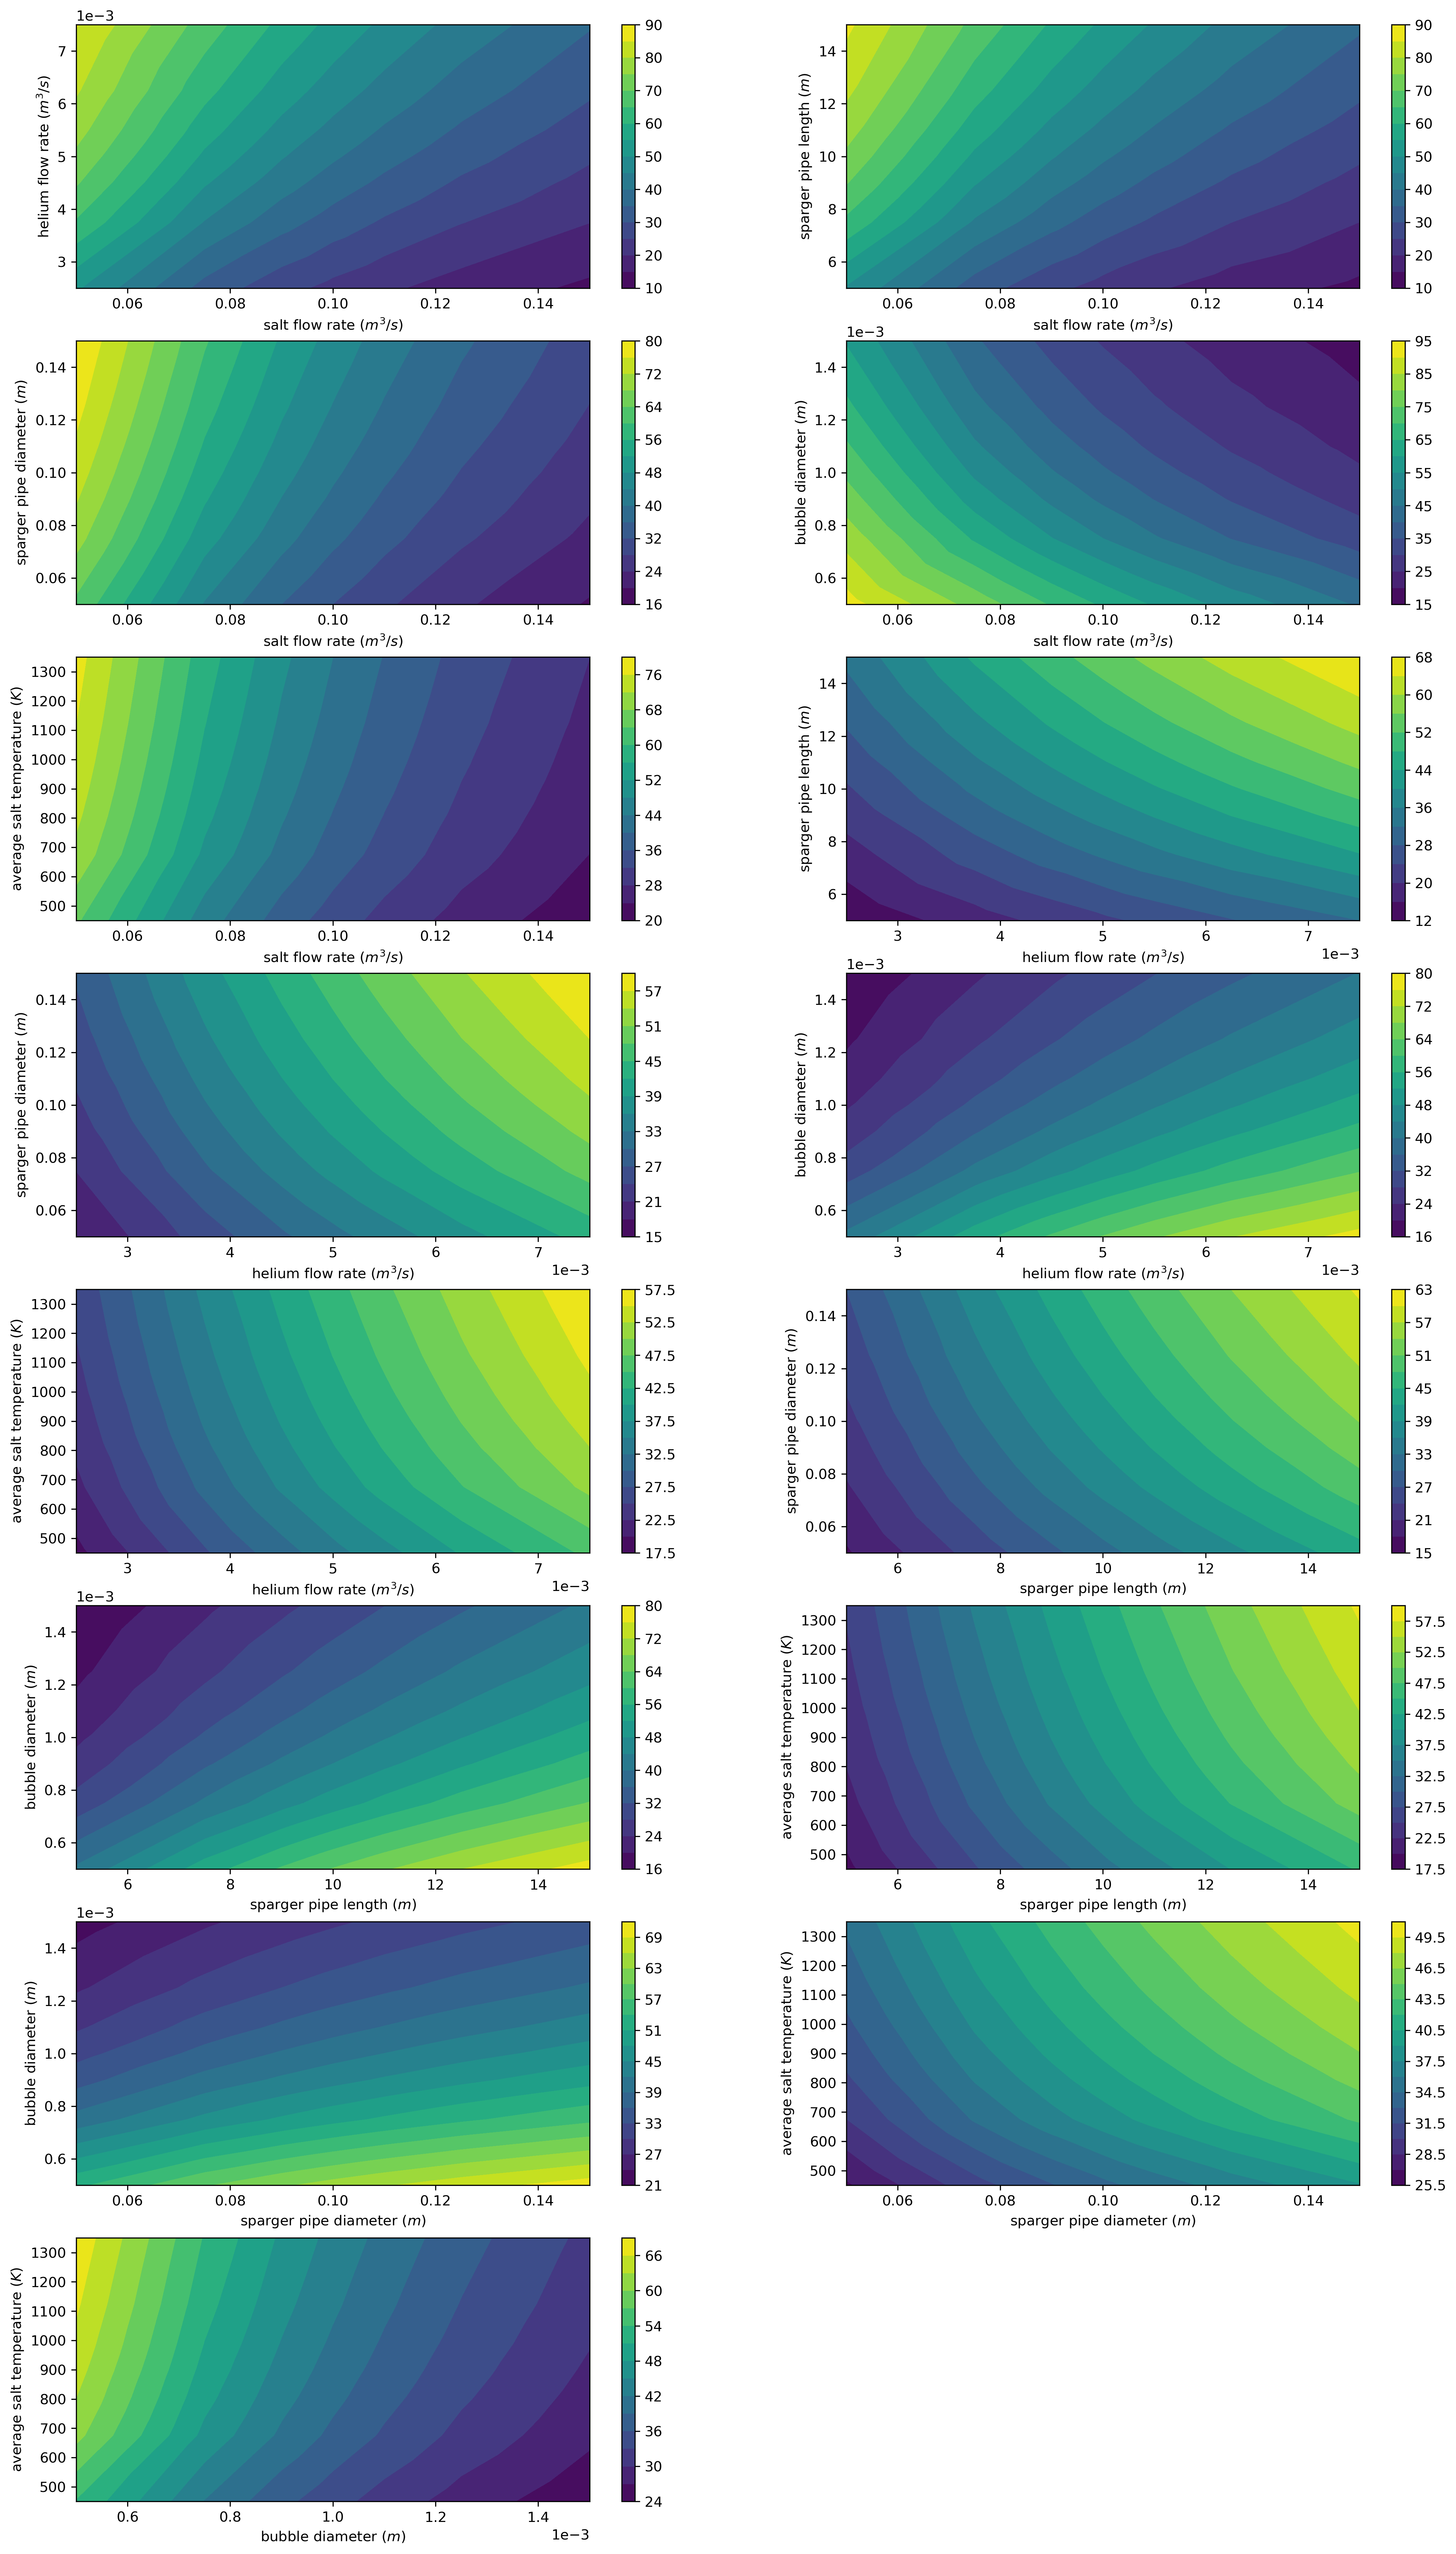
\includegraphics[width=0.8\textwidth]{Sparger_result.png}
        \end{center}
        \caption{Binary effect of design parameters on the Xe removal 
            efficiency ($\varepsilon$$_{Xe}$).}
        \label{fig:binary_eff_sparger}
    \end{figure}

\newpage
\FloatBarrier

\subsubsection{Separator Design}

    Similar to the sparger case, we sought potential separator designs around 
    its base design and changed the considered parameters of the base design up 
    to $\pm$ 50\%. Figure \ref{fig:individual_eff_separator} and 
    \ref{fig:binary_eff_separator} show the effects of these parameters on the 
    bubble separation efficiency. Note that since the presented efficiency is 
    associated with the separation of bubbles from the salt (not with the 
    transfer of target elements), all target isotopes must have the same value.

    From the binary effects, as in the sparger case, all parameters are 
    independent variables. The only convex-like structure is seen in the 
    subplot of average salt temperature versus pipe diameter. But, we think 
    this is because these two parameters are the most critical players on 
    efficiency and their effects are at great amounts when their values are 
    changed slightly.

    According to the results of individual effects, gas removal efficiency 
    increases with increasing salt flow rate, helium flow rate, gas outlet 
    diameter, bubble diameter, and salt temperature whereas it decreases with 
    increasing pressure difference and pipe diameter.

    Among these parameters, the salt temperature cannot be lower than 800 K due 
    to the solidification concerns on the salt at low temperatures.

    Pressure difference and helium flow rate parameters seem insignificant on 
    the separation efficiency. The most important player is the pipe diameter 
    that directly affects the flow dynamics.

    As discussed in Milestone 1.2 for the effect of bubble diameter on the 
    separator, bubble diameter has to be around 1 mm because both sparger and 
    separator are influenced by it. The smaller the bubble diameter the sparger 
    has, the higher gas removal efficiency the sparger yields. Oppositely, the 
    smaller bubble diameter the separator has, the lower bubble separation 
    efficiency the separator yields.

    In any case, we stayed above 95\% bubble separation efficiency while the 
    base design yields about 99\% efficiency.

\begin{figure}[htbp!]
    \begin{center}
        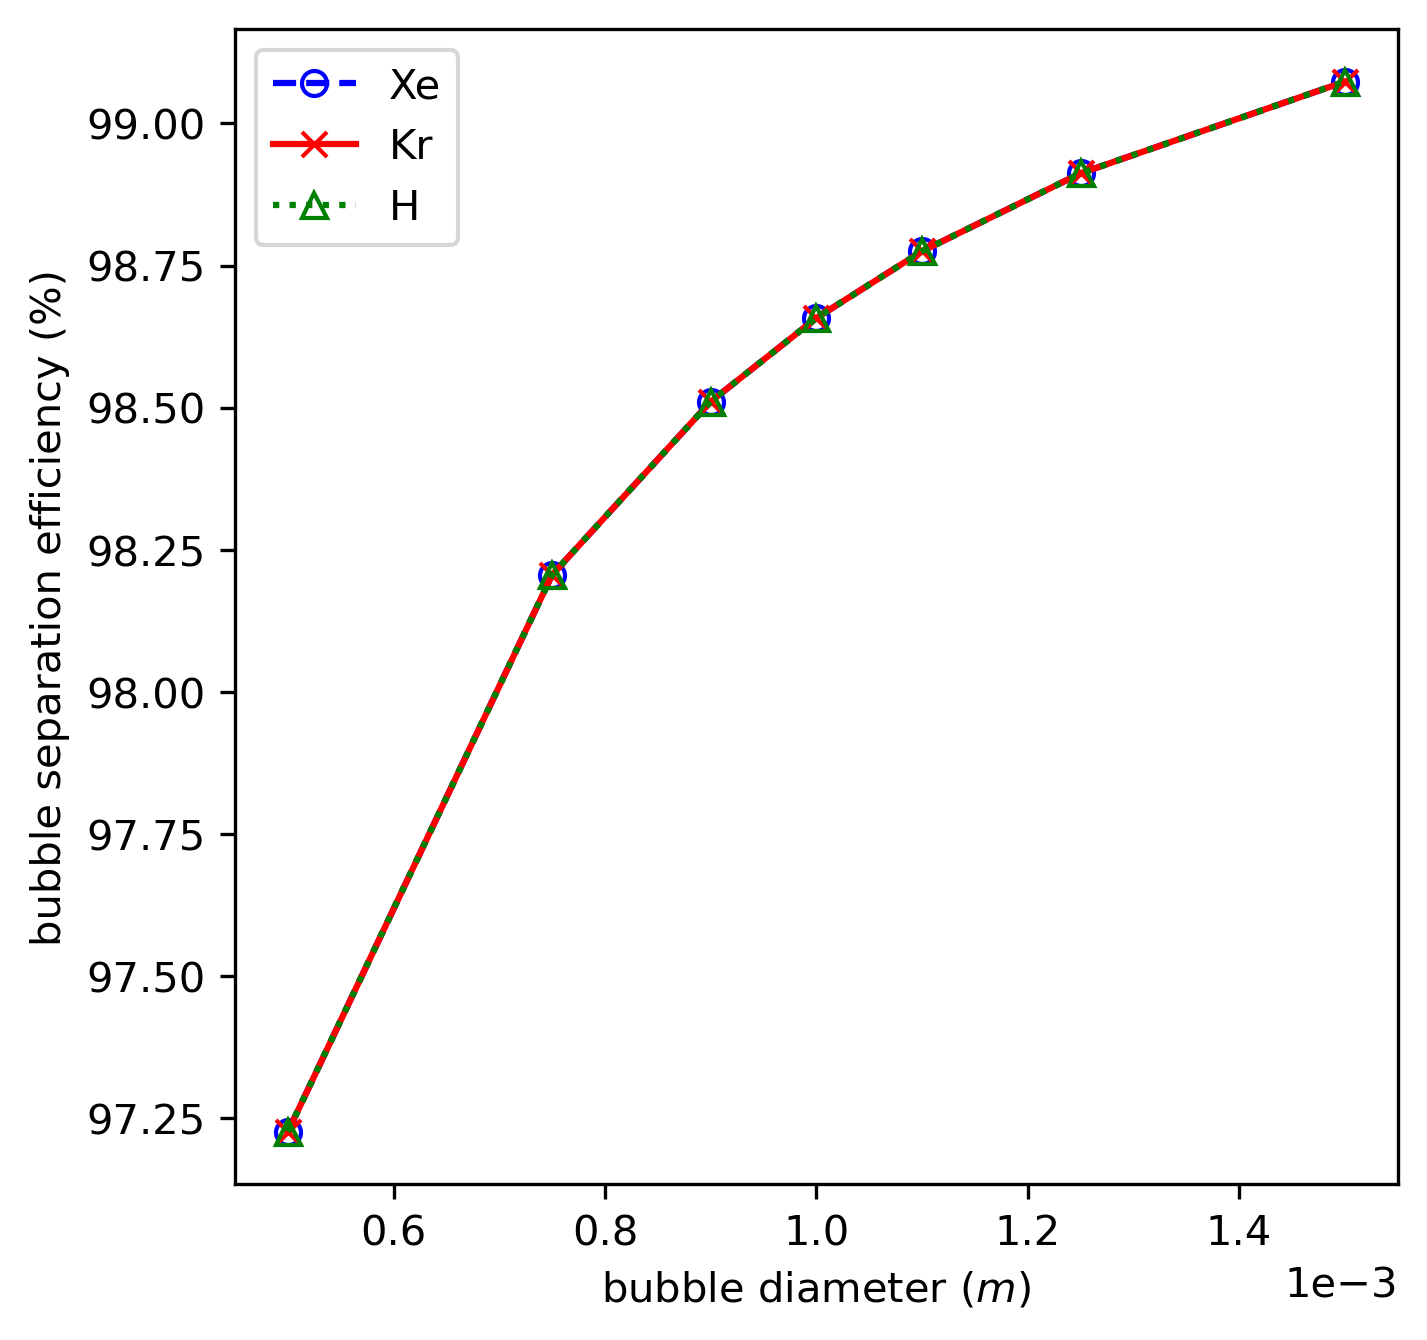
\includegraphics[width=0.4\textwidth]{Separator_sep_eff_vs_db.png}
        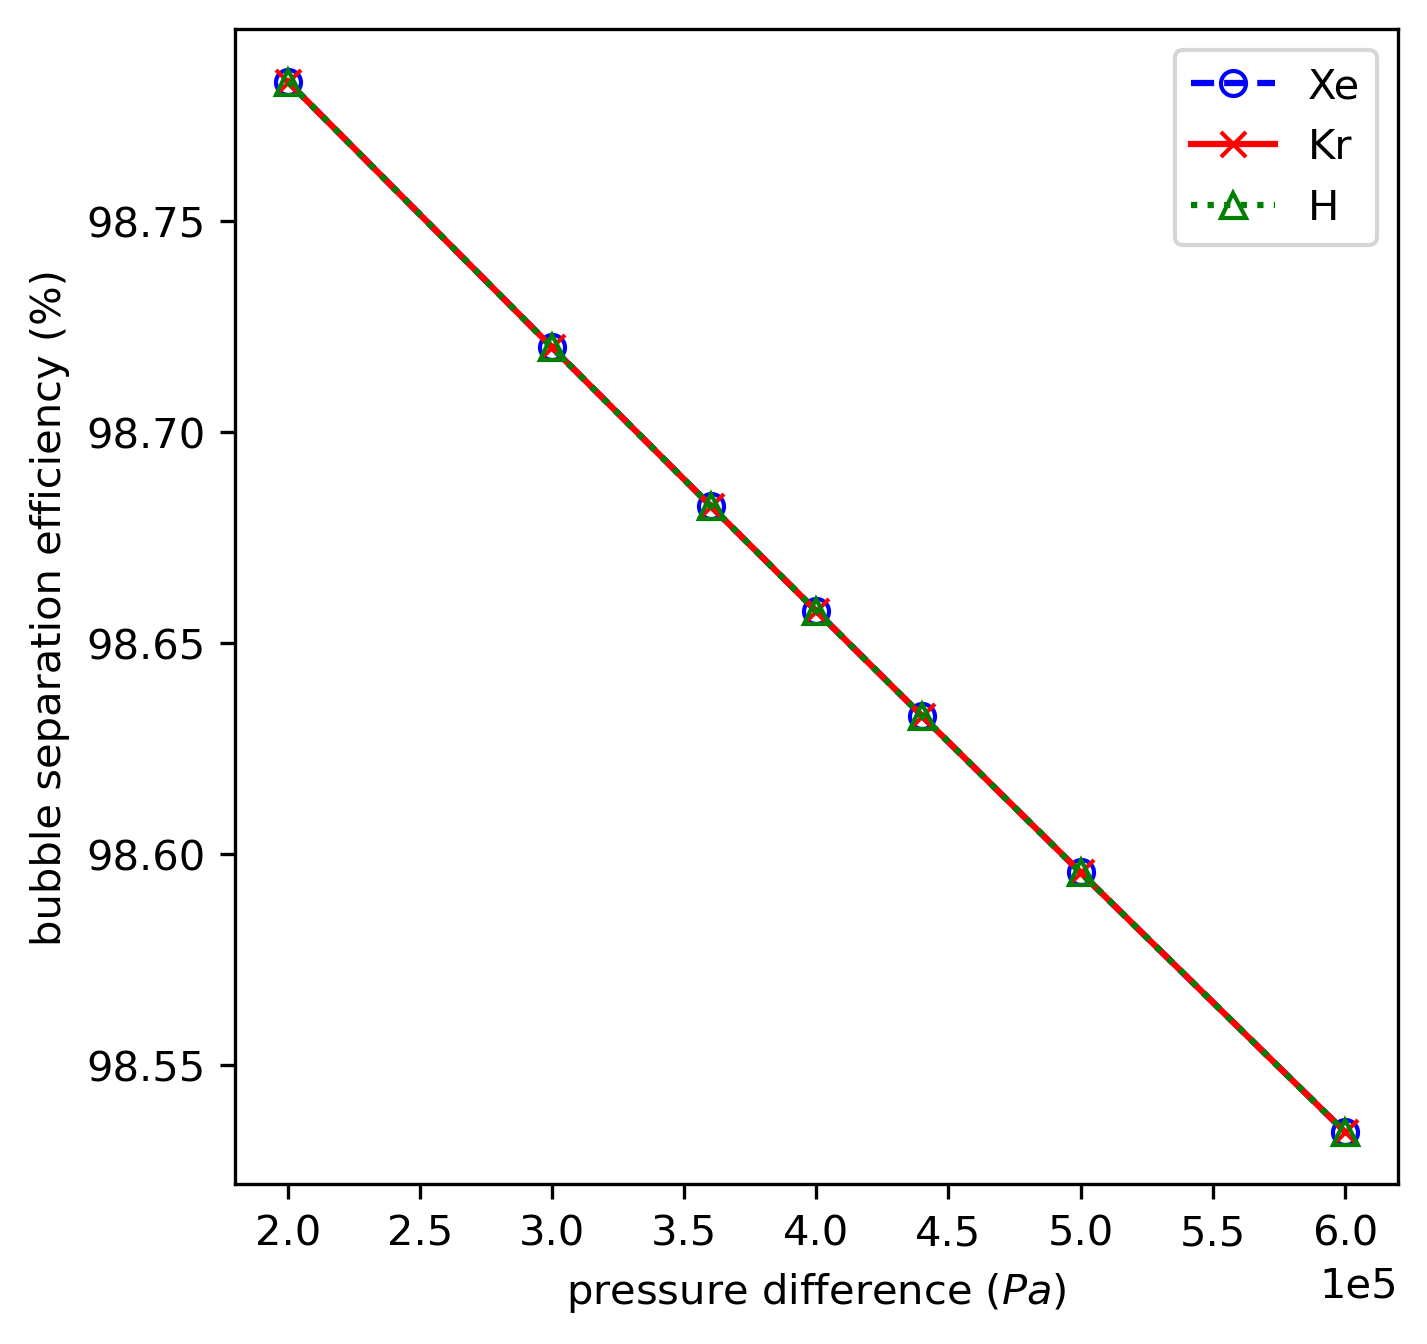
\includegraphics[width=0.4\textwidth]{Separator_sep_eff_vs_deltap.png}
        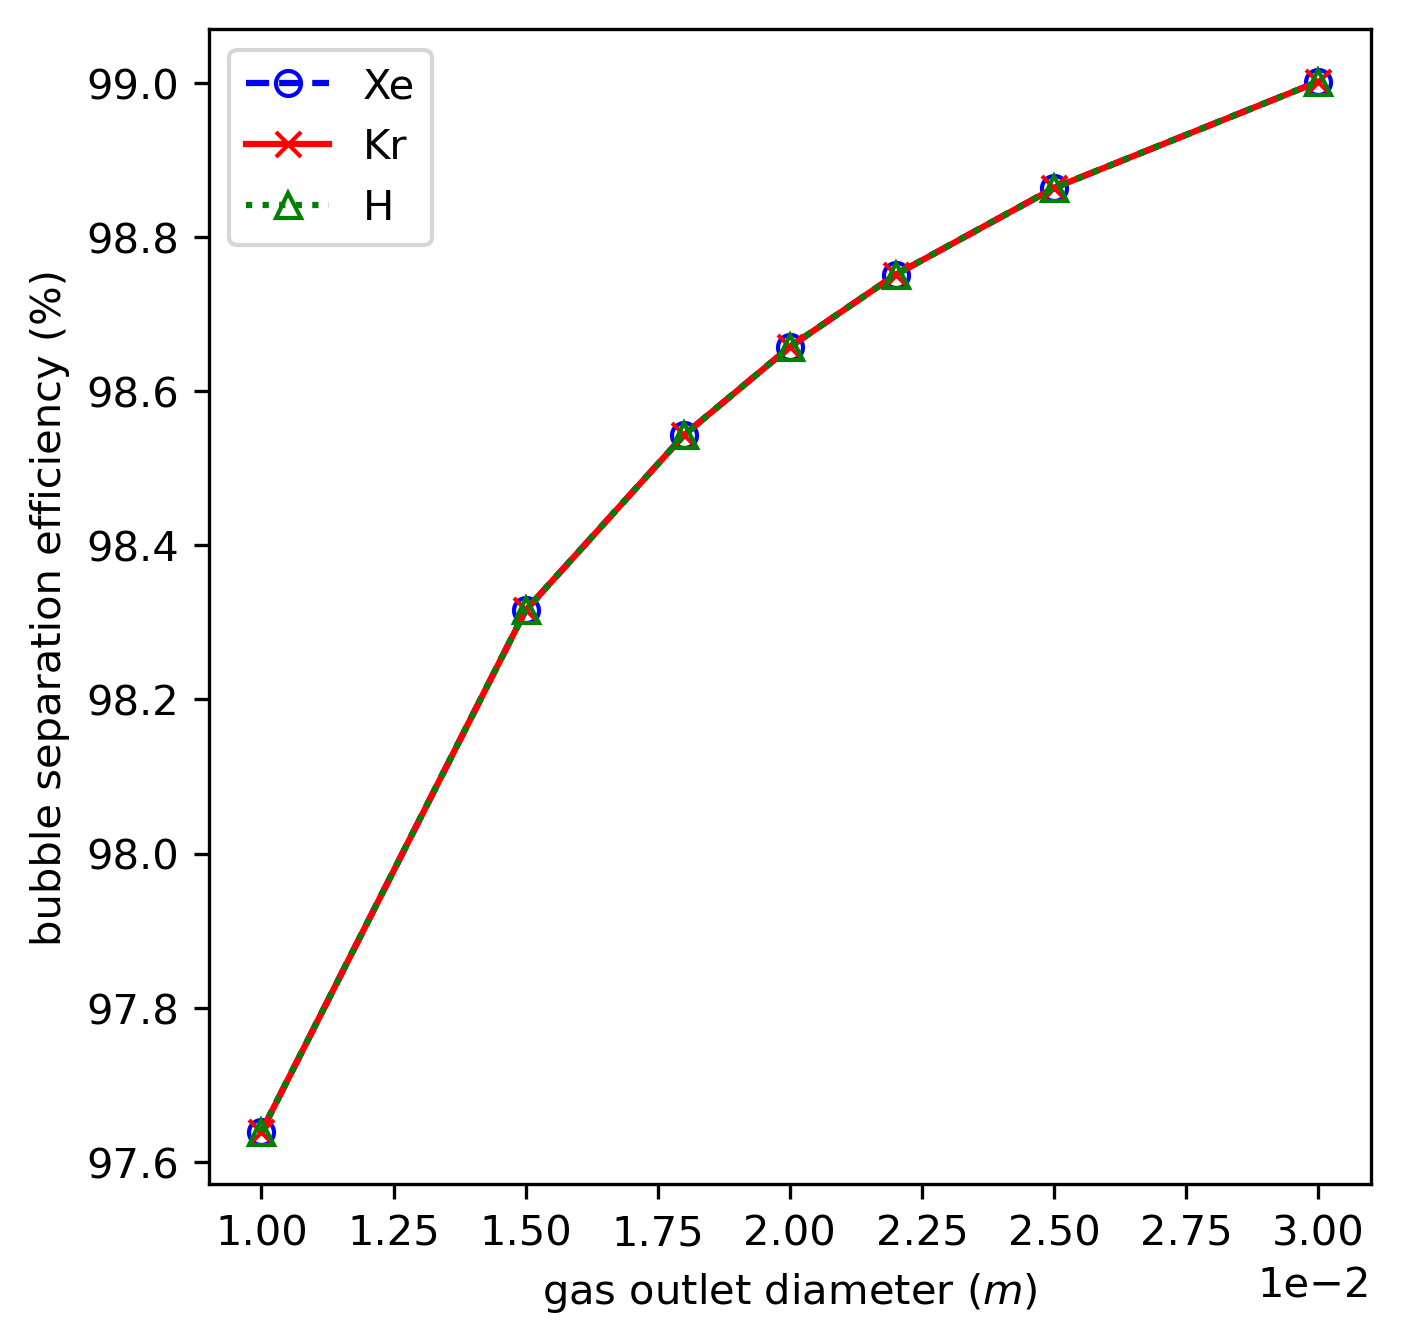
\includegraphics[width=0.4\textwidth]{Separator_sep_eff_vs_do.png}
        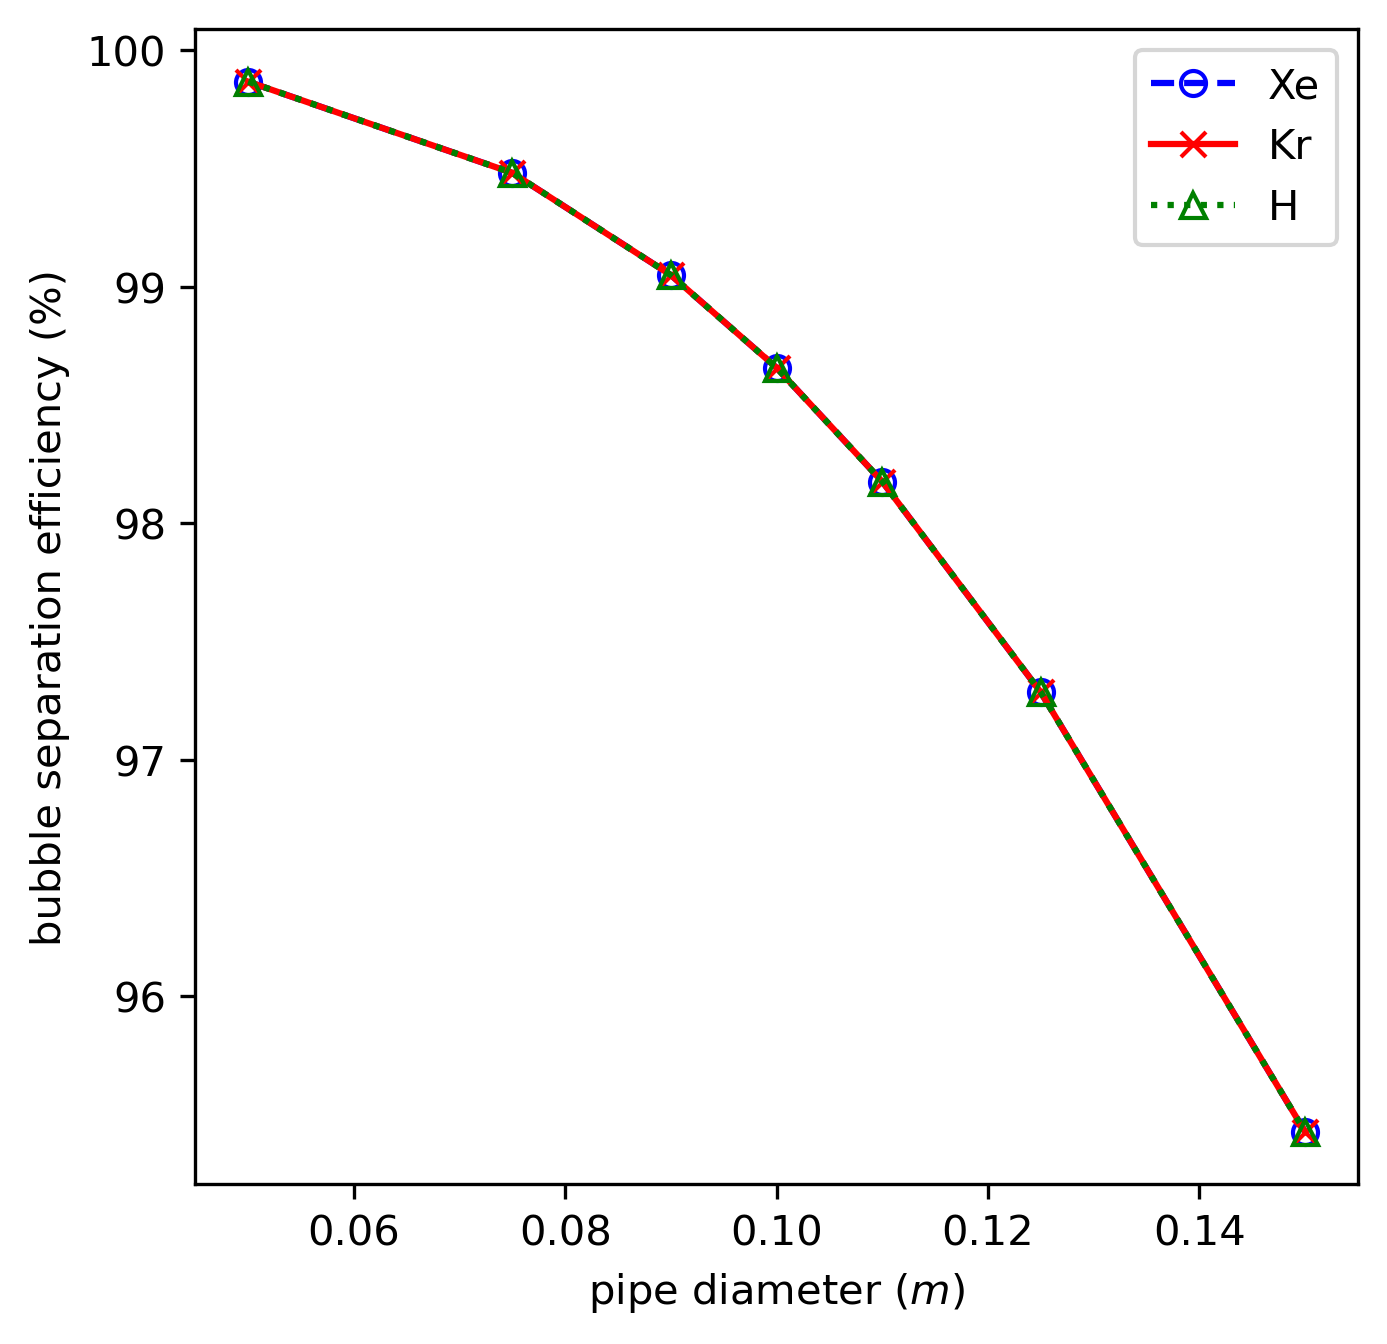
\includegraphics[width=0.4\textwidth]{Separator_sep_eff_vs_dp.png}
        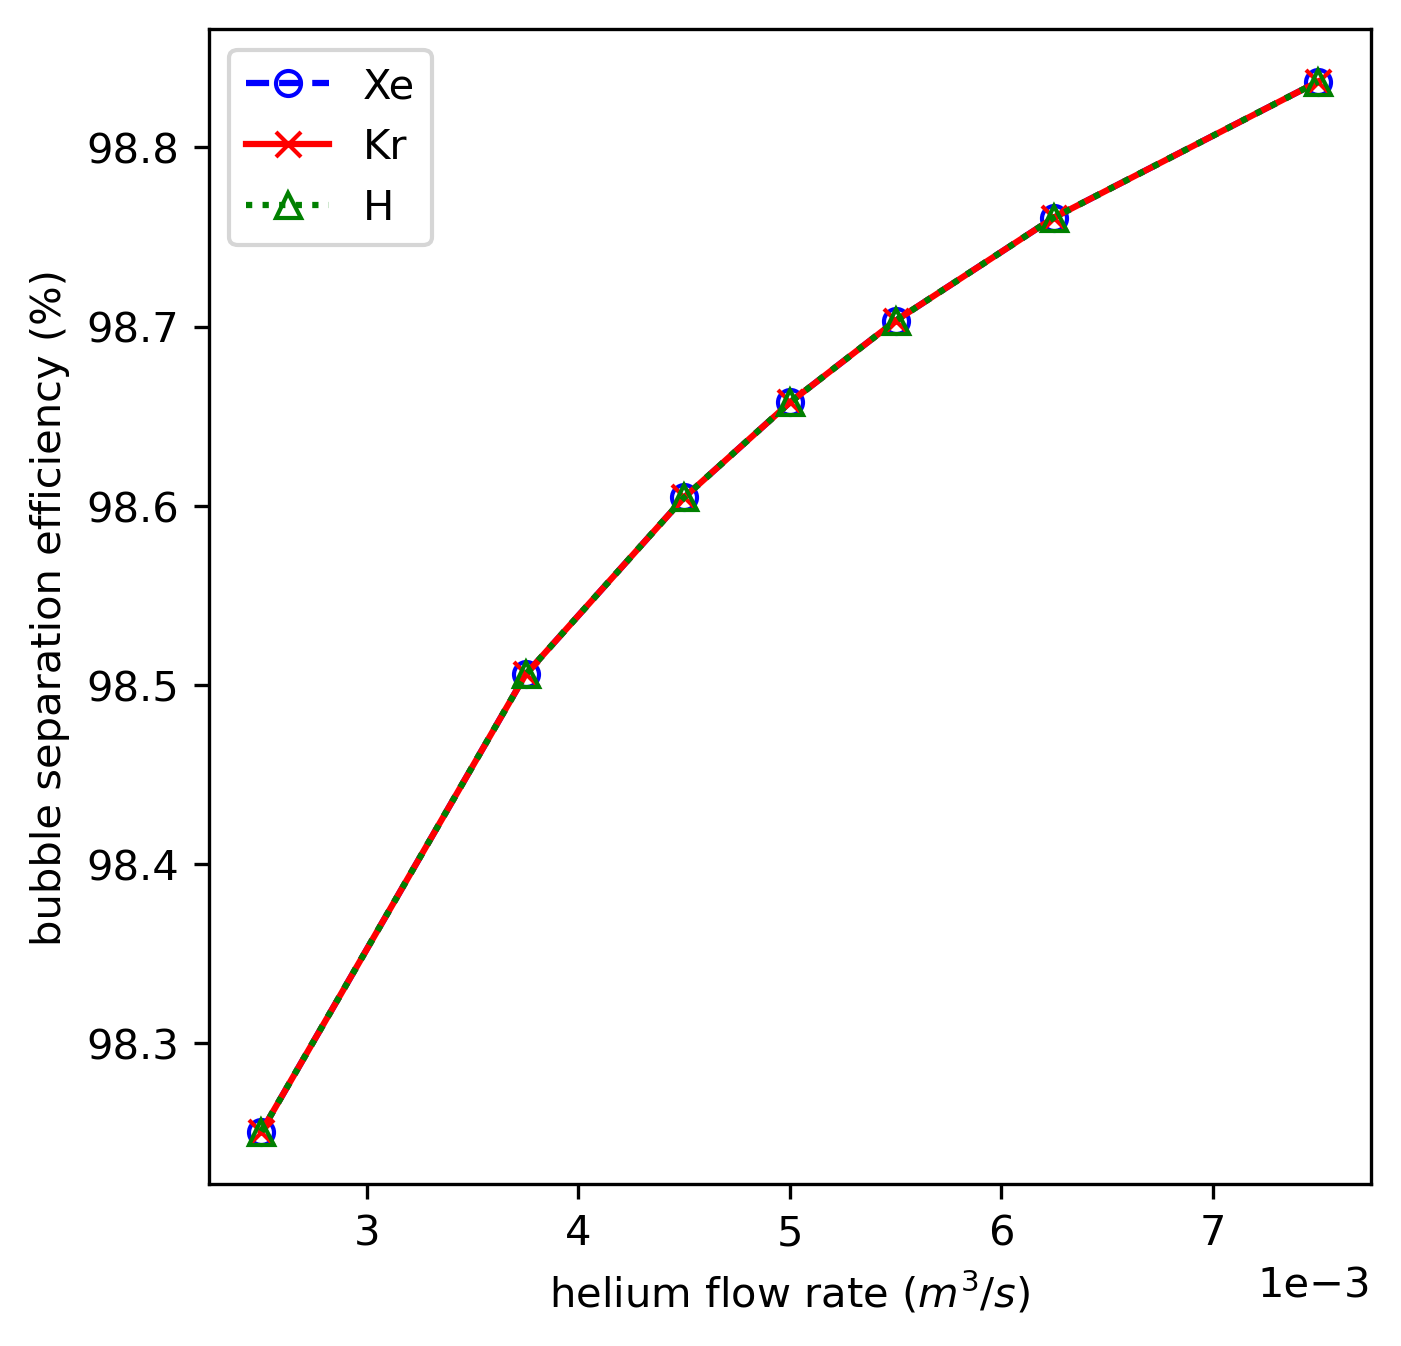
\includegraphics[width=0.4\textwidth]{Separator_sep_eff_vs_q_he.png}
        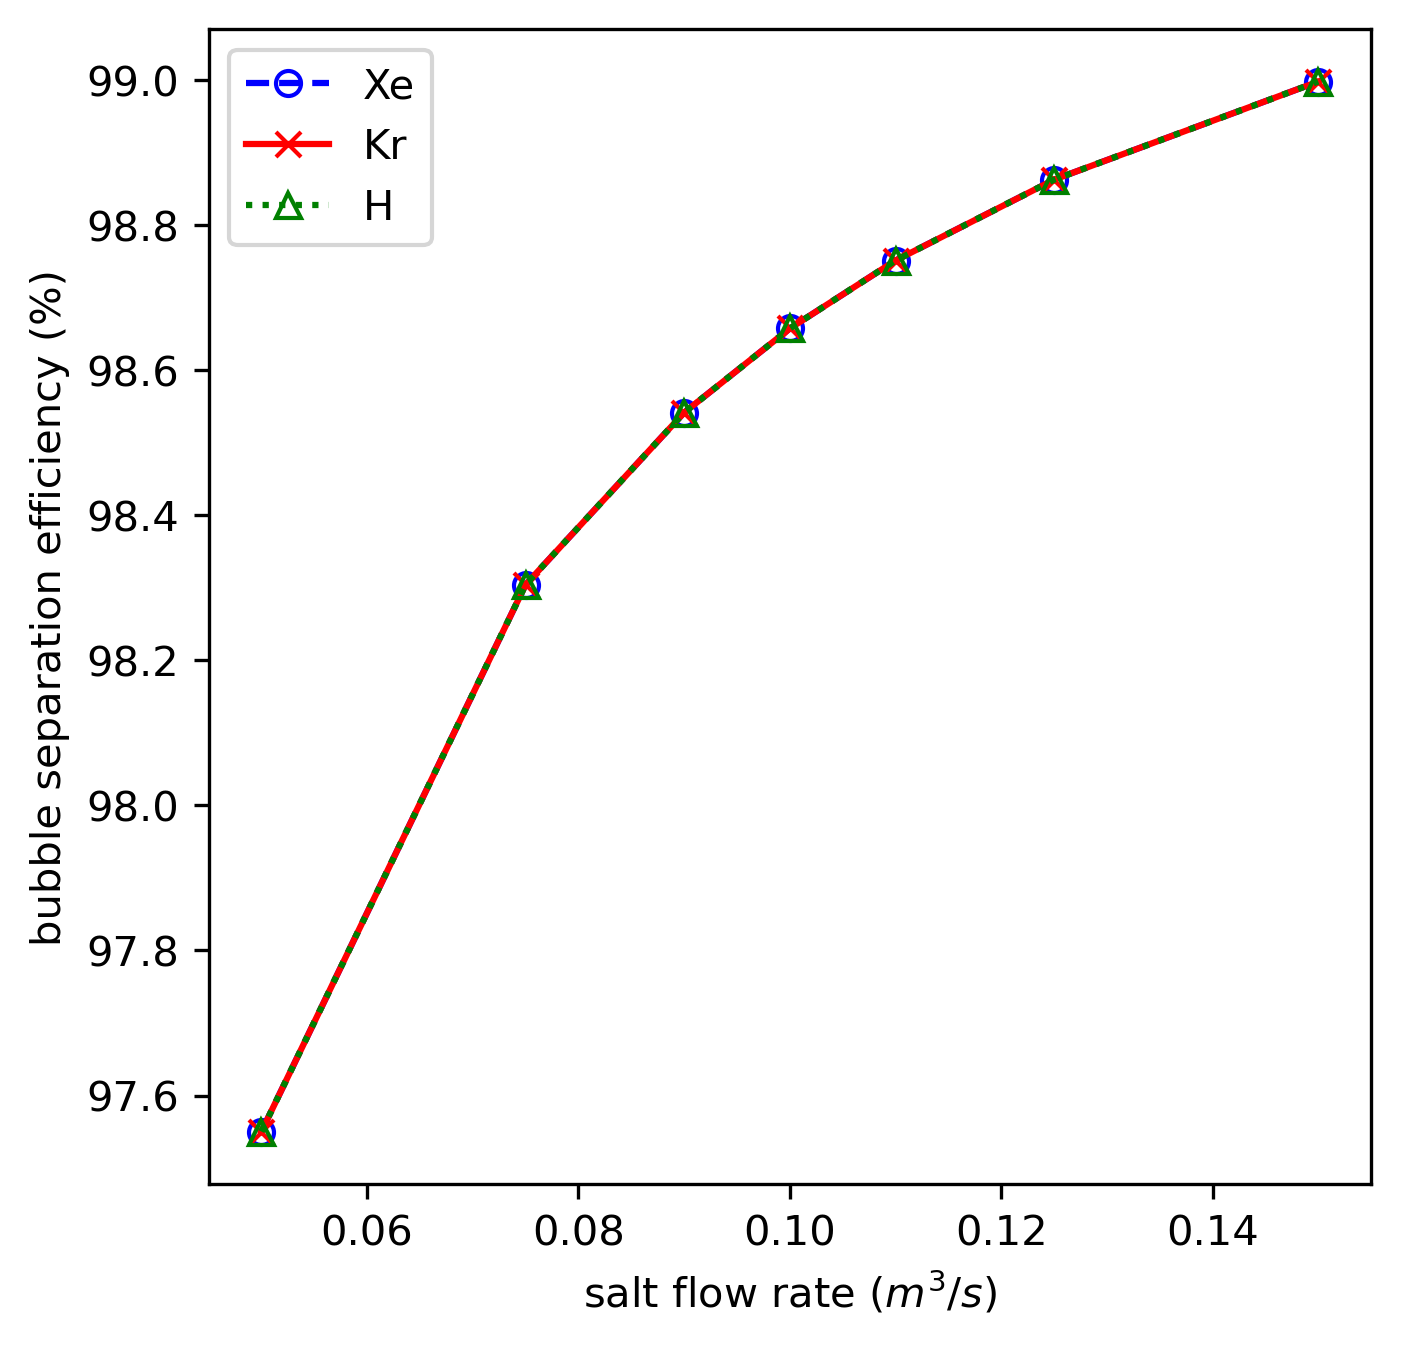
\includegraphics[width=0.4\textwidth]{Separator_sep_eff_vs_q_salt.png}
        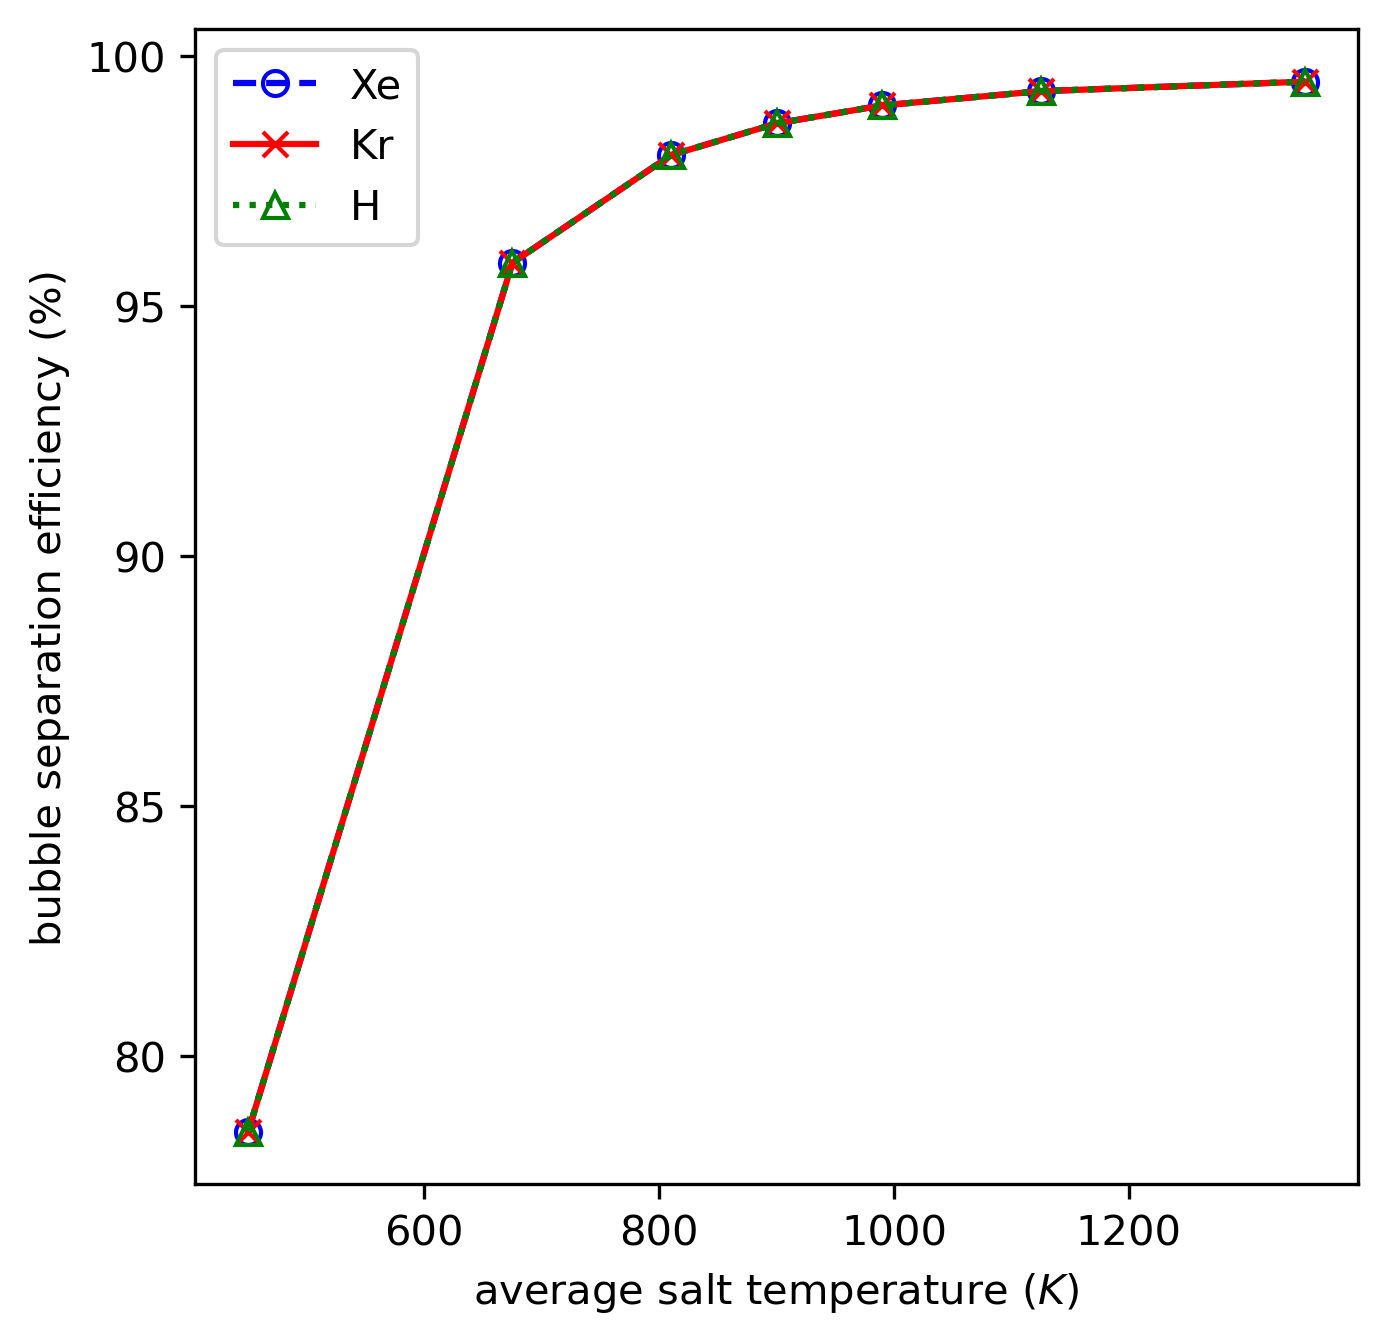
\includegraphics[width=0.4\textwidth]{Separator_sep_eff_vs_temp_salt.png}
    \end{center}
    \caption{Individual effect of design parameters on the bubble separation 
        efficiency ($\varepsilon$$_{sep}$).}
    \label{fig:individual_eff_separator}
\end{figure}

\begin{figure}[htbp!]
    \begin{center}
        \includegraphics[width=0.7\textwidth]{Separator_result.png}
    \end{center}
    \caption{Binary effect of design parameters on the bubble separation
    efficiency ($\varepsilon$$_{sep}$).}
    \label{fig:binary_eff_separator}
\end{figure}

\newpage
\FloatBarrier

\section{Conclusion}

    In short, MSBR can, without difficulty, operate under load follow transient 
    with low gas removal efficiency, unless the shutdown period is too long, 
    typically greater than 4 hours. Recovery time depends directly on gas 
    removal efficiency and load-follow period. From the results of the first 
    part, we would need an adjustable sparger/separator design to achieve 
    sufficient gas removal for all kinds of load-follow scenarios.

    From the binary effects of the design parameters of sparger and separator, 
    each design parameter has no relation with the other parameters, acting 
    like a free variable and affecting the removal/separation efficiency 
    independently.

    We can use the separator base design which yields 98.7\% efficiency for the 
    pipe diameter ($d_p$) = 0.1 m, bubble diameter ($d_b$) = 1 mm, salt 
    volumetric flow rate ($Q_{salt}$) = 0.1 m$^{3}$/s, salt temperature 
    ($T_{salt}$) = 900 K, pressure difference ($\Delta p$) = 4e5 Pa, gas outlet 
    diameter ($D_o$) = 0.02, and helium volumetric flow rate ($Q_{He}$) = 0.005 
    m$^{3}$/s. These design features are well sufficient.

    On the other hand, it seems the separator design is not critical as its 
    efficiency is always above 95\%. Even if we change the separator design 
    parameters by half, the change in the efficiency seems to remain very 
    limited with a few percent change. Therefore, these results indicate that 
    the main difficulty in designing sparging system comes from nothing but the 
    sparger component. It has to be designed according to the removal 
    efficiency imposed by the reactor core. Note that one of the important 
    design parameters which are affecting both sparger and separator is bubble 
    diameter as pointed out in Milestone 1.2.

    The base design which provides an $\varepsilon$$_{Xe}$ of about 40\% may be 
    a good starting point in designing a sparging system. This design seems 
    sufficient in particular for the reactor cores which need less than 40\% 
    gas removal efficiency to compensate the reactivity loss due to Xe 
    poisoning. On the other hand, we need a more adaptable sparger design for a 
    prompt response to a need for a higher gas removal efficiency like 
    $\varepsilon$$_{Xe}$ = 0.769 as indicated in Figure \ref{fig:triple_keff}. 
    In this manner, we are recommending a few sparger designs (for the 
    worst-case scenarios) below: one for $\varepsilon$$_{Xe}$ = 53.6 and one 
    for $\varepsilon$$_{Xe}$ = 76.9\%.

    To reach at the goal of $\varepsilon$$_{Xe}$ = 53.6 implied by Figure 
    \ref{fig:double_keff} for the double load follow transient, it would be 
    sufficient to increase only sparger pipe length and diameter by 30\% in the 
    base design, without touching the gas and salt flow rates. That is, the 
    sparger design should have a pipe length (L) = 13 m, pipe diameter ($d$) = 
    0.13 m, bubble diameter ($d_b$) = 1 mm, salt volumetric flow rate 
    (Q$_{salt}$) = 0.1 m$^{3}$/s, salt temperature ($T_{salt}$) = 900 K and 
    helium volumetric flow rate (Q$_{He}$) = 0.005 m$^{3}$/s.

    In the case of reaching at the goal of $\varepsilon$$_{Xe}$ = 76.9\% 
    implied by Figure \ref{fig:triple_keff} for the triple load follow 
    transient, it would not be as easy as to go the goal of 
    $\varepsilon$$_{Xe}$ = 53.6\%. This is because there is no way to go to 
    76.9\% even if we increase the sparger pipe length and diameter by 50\%. 
    Therefore we need additional parameters to adjust. Changing the gas to salt 
    flow rate ratio seems the only way as the other parameters have a very 
    limited impact on the efficiency to increase. In this manner, increasing 
    the gas flow rate and sparger pipe length and diameter by 50\% in the base 
    design yields the required efficiency. That is, the sparger design should 
    have a pipe length (L) = 15 m, pipe diameter ($d$) = 0.15 m, bubble 
    diameter ($d_b$) = 1 mm, salt volumetric flow rate (Q$_{salt}$) = 0.1 
    m$^{3}$/s, salt temperature ($T_{salt}$) = 900 K and helium volumetric flow 
    rate (Q$_{He}$) = 0.0075 m$^{3}$/s.

    It appears from the results that the best option is to regulate the gas 
    flow rate and/or salt flow rate during operation, or much better is to 
    balance the ratio (by less than 5\%) of gas flow rate to salt flow rate, 
    which is delimited by thermal-hydraulic effects. Another good option is to 
    make the sparger pipe length longer as efficiency reacts equally to change 
    in length, like 10\% for 10\%. It also has no significant effect on the 
    separator.

    To sum up, the main findings in this milestone are: (i) TAP can do 
    load-following without gas removal and safety parameters remained almost 
    constant, (ii) MSBR needs gas removal for the load-following but very high 
    separation efficiency is unnecessary, (iii) We need an adaptable sparging 
    design so that a sufficient gas removal is achievable for all kinds of 
    load-follow scenarios, and (iv) design parameters are very limited by the 
    flow dynamics and core requirements.


\bibliographystyle{unsrt}
\bibliography{bibliography}
\end{document}

